\documentclass{jcse}

\usepackage{url}
\usepackage{amsmath}
\usepackage{amssymb}
\usepackage{flushend}
\usepackage{booktabs}
\usepackage{graphicx}
\usepackage{algorithm}
\usepackage{algpseudocode}
\usepackage{cite}

\papertype{Regular Paper}
\papertypeAtFoot{Open Access}
\volumeyear{Jan 0000} \volumenumber{00} \issuenumber{0} \pp{000-000}
\DOI{yy.5626/JCSE.2011.5.2.xxx}

\received{00 Month 2011}
\revised{00 Month 2011}
\accepted{00 Month 2011}

\permissionUrl{http://jcse.kiise.org}

\copyrightString{Copyright \textcopyright 2011. The Korean Institute of Information Scientists and Engineers}

\issn{pISSN: 1976-4677 eISSN: 2093-8020}

\permission{
This is an Open Access article distributed under the terms of the Creative Commons Attribution Non-Commercial License (\url{http://creativecommons.org/licenses/
by-nc/3.0/}) which permits unrestricted non-commercial use, distribution, and reproduction in any medium, provided the original work is properly cited.
}

\renewcommand{\arraystretch}{0.92}

\setcounter{topnumber}{4}
\setcounter{bottomnumber}{4}
\setcounter{totalnumber}{6}
\setcounter{dbltopnumber}{3}
\renewcommand{\topfraction}{0.95}
\renewcommand{\bottomfraction}{0.95}
\renewcommand{\textfraction}{0.05}
\renewcommand{\floatpagefraction}{0.85}
\renewcommand{\dbltopfraction}{0.95}
\renewcommand{\dblfloatpagefraction}{0.85}

\setlength{\textfloatsep}{4pt plus 1.0pt minus 1.0pt}
\setlength{\floatsep}{4pt plus 1.0pt minus 1.0pt}
\setlength{\intextsep}{5pt plus 1.0pt minus 1.0pt}
\setlength{\dbltextfloatsep}{5pt plus 1.0pt minus 1.0pt}
\setlength{\dblfloatsep}{5pt plus 1.0pt minus 1.0pt}

\title[Localizing INT8 Quantization Collapse and Channel Pruning on Edge]{Localizing INT8 Quantization Collapse and Channel Pruning for Resilient Edge Poultry Disease Diagnosis}

\author{
	\authname{Fatih Jawwad Al Mumtaz$^*$} \\
	\affaddr{Department of Informatics, Faculty of Science and Technology, Universitas Darussalam Gontor, Ponorogo 63471, Indonesia} \\
	\email{fatihalmumtaz76@student.cs.unida.gontor.ac.id} \\
	\\
	\authname{Farrel Ghozy Afifuddin} \\
	\affaddr{Department of Informatics, Faculty of Science and Technology, Universitas Darussalam Gontor, Ponorogo 63471, Indonesia} \\
	\email{farrelaffifudin@student.cs.unida.gontor.ac.id} \\
}
\shortauthors{F. J. Al Mumtaz and F. G. Afifuddin}

\bottomstuff{
$^*$ Corresponding Author: Fatih Jawwad Al Mumtaz (Email: fatihalmumtaz76@student.cs.unida.gontor.ac.id; Tel: +62-851-4339-6221).
}

\category{Embedded Computing}

\keywords{Edge Artificial Intelligence, post-training quantization collapse, structured channel pruning, depthwise separable convolution, embedded vision, Raspberry Pi 5, precision livestock farming.}

\begin{document}

\maketitle

\begin{abstract}
Deploying lightweight convolutional neural networks on micro-edge embedded devices is critical for automated precision poultry disease surveillance in low-connectivity rural agricultural facilities. However, post-training INT8 quantization—the prevailing edge compression standard—exhibits catastrophic accuracy failure on depthwise-separable topologies. In this paper, we localize, mathematically diagnose, and mitigate this quantization collapse across MobileNetV2, ShuffleNetV2, and EfficientNet-B0 on a verified leak-free dataset. First, an algorithmic perceptual hash audit ($D_H \le 5$) of published poultry benchmarks uncovered 617 near-duplicate pairs (including 156 cross-partition train-test duplicates), establishing an empirical optimistic evaluation bias (+0.15\% to +0.39\% overall accuracy with 100\% recall on duplicate frames). Decontaminating the benchmark yielded an 8,153-image sterile dataset containing 1,728 isolated test images. While dynamic INT8 preserves MobileNetV2 at 97.11\% and ShuffleNetV2 at 97.45\%, it induces catastrophic collapse in EfficientNet-B0 from 98.55\% down to 10.42\%, where 97.0\% of predictions degenerate into Newcastle Disease. Layer-wise signal-to-quantization-noise ratio (SQNR) analysis reveals that depthwise separable convolutions exhibit extreme cross-channel weight dynamic range ($\Delta_w \approx 14.8$), restricting effective bit-width to $B_{\text{eff}} \le 4.09$ bits and driving depthwise SQNR down to 8.4\,dB under per-tensor scaling. We formulate a static per-channel Quantize-Dequantize (QDQ) calibration protocol that universally recovers all architectures: EfficientNet-B0 to 94.56\% ($p < 10^{-15}$, paired McNemar test), MobileNetV2 to 97.74\% (94.33\% Newcastle recall), and ShuffleNetV2 to 97.57\% (94.33\% Newcastle recall). Furthermore, structured channel pruning reveals that unweighted cross-entropy loss starves the lethal minority class, driving Newcastle Disease recall from 94.33\% down to 31.21\% at 50\% sparsity; we demonstrate that class-weighted loss with FP32 knowledge distillation counteracts this starvation. Physical profiling on a Raspberry Pi 5 ARM Cortex-A76 under ONNX Runtime 1.29 CPU Execution Provider shows that uncompressed FP32 models execute natively in real time (51.33 to 110.69 FPS), demonstrating that compression is unneeded on high-end 8\,GB SBCs but critical for micro-edge tiers (e.g., Pi Zero 2 W). Dynamic INT8 expands operator execution from 55 fused nodes to 357 disjoint nodes, incurring a 2.16$\times$ to 2.39$\times$ slowdown. Conversely, static QDQ fuses into native \texttt{QLinearConv} leveraging Cortex-A76 \texttt{dotprod} NEON vector instructions, accelerating MobileNetV2 to 7.53\,ms (132.8 FPS, 2.65$\times$ speedup), ShuffleNetV2 to 6.12\,ms (163.5 FPS, 1.57$\times$ speedup), and EfficientNet-B0 to 19.04\,ms (52.5 FPS, 1.94$\times$ speedup).
\end{abstract}

\section{Introduction}
Avian infectious pathologies, notably Coccidiosis, Salmonella, and Newcastle Disease, pose severe economic risks and global food security challenges across commercial and smallholder poultry facilities \cite{machuve2021poultry,dianyo2022fecal}. In rural livestock farms, continuous clinical veterinary inspection is cost-prohibitive, leading to delayed disease identification and rapid flock-wide mortality. To overcome these logistical barriers, automated visual diagnostic systems operating directly on edge embedded micro-nodes, such as low-cost single-board computers situated within coop perimeters, have emerged as a vital precision agriculture paradigm. Edge inference eliminates dependence on intermittent cloud connectivity, safeguards biosecurity data privacy, and provides instantaneous diagnostic feedback.

While high-performance edge single-board computers (such as the Raspberry Pi 5 with 8\,GB LPDDR4X RAM) possess sufficient memory bandwidth to execute uncompressed FP32 models in real time (exceeding 50 to 110 FPS), deployable micro-edge agricultural monitoring nodes (such as the Raspberry Pi Zero 2 W with 512\,MB RAM or low-power embedded microcontrollers) operate under stringent hardware constraints characterized by limited SRAM, restricted thermal envelopes, and tight electrical power budgets \cite{jacob2018quantization,wu2019tinyml}. On such resource-constrained micro-edge tiers, aggressive model compression through post-training quantization and channel pruning is indispensable to fit model weights into limited caches and minimize memory-bus energy. Eight-bit integer (INT8) quantization represents the prevailing industry standard for edge deployment, typically delivering a fourfold reduction in model storage footprint and accelerating matrix multiplication routines through integer vector ALUs.

While INT8 post-training quantization is widely assumed to incur negligible accuracy loss ($< 1\%$) on traditional over-parameterized convolutional networks such as ResNet, compact parameter-efficient architectures often exhibit fragile numerical characteristics. In particular, we demonstrate that EfficientNet-B0 \cite{tan2019efficientnet} undergoes catastrophic quantization collapse when quantized naively using standard dynamic 8-bit integer formats. Its top-1 diagnostic accuracy plummets precipitously from 98.55\% in 32-bit floating-point (FP32) precision down to 10.42\% in INT8 precision, rendering the autonomous diagnostic system completely unusable. This failure occurs silently, producing confident but uniformly erroneous diagnostic classifications across all clinical disease categories.

In this paper, we conduct a systematic empirical and theoretical investigation that isolates, mathematically diagnoses, and mitigates post-training quantization collapse on compact vision models. Fig.~\ref{fig:pipeline} illustrates our complete methodological pipeline. We first establish a rigorous experimental foundation by conducting a perceptual hash audit on widely cited public poultry datasets, quantifying leakage effect size and removing duplicate image pairs that introduce optimistic evaluation bias. We subsequently formulate the signal-to-quantization-noise ratio (SQNR) across network layers, demonstrating that severe cross-channel weight variance in depthwise separable convolutions is the primary driver of numerical degradation. 

To resolve this limitation, we develop a static per-channel Quantize-Dequantize calibration protocol that restores diagnostic fidelity across all architectures without requiring expensive retraining. We further explore the interaction between structured channel pruning and integer quantization, identifying how unweighted loss starves minority lethal classes and validating class-weighted knowledge distillation. Finally, we benchmark all configurations on a physical Raspberry Pi 5 embedded system, analyzing execution latency, native vector instruction acceleration, multithreading efficiency, and off-grid battery autonomy.

\begin{figure}[t]
\centering
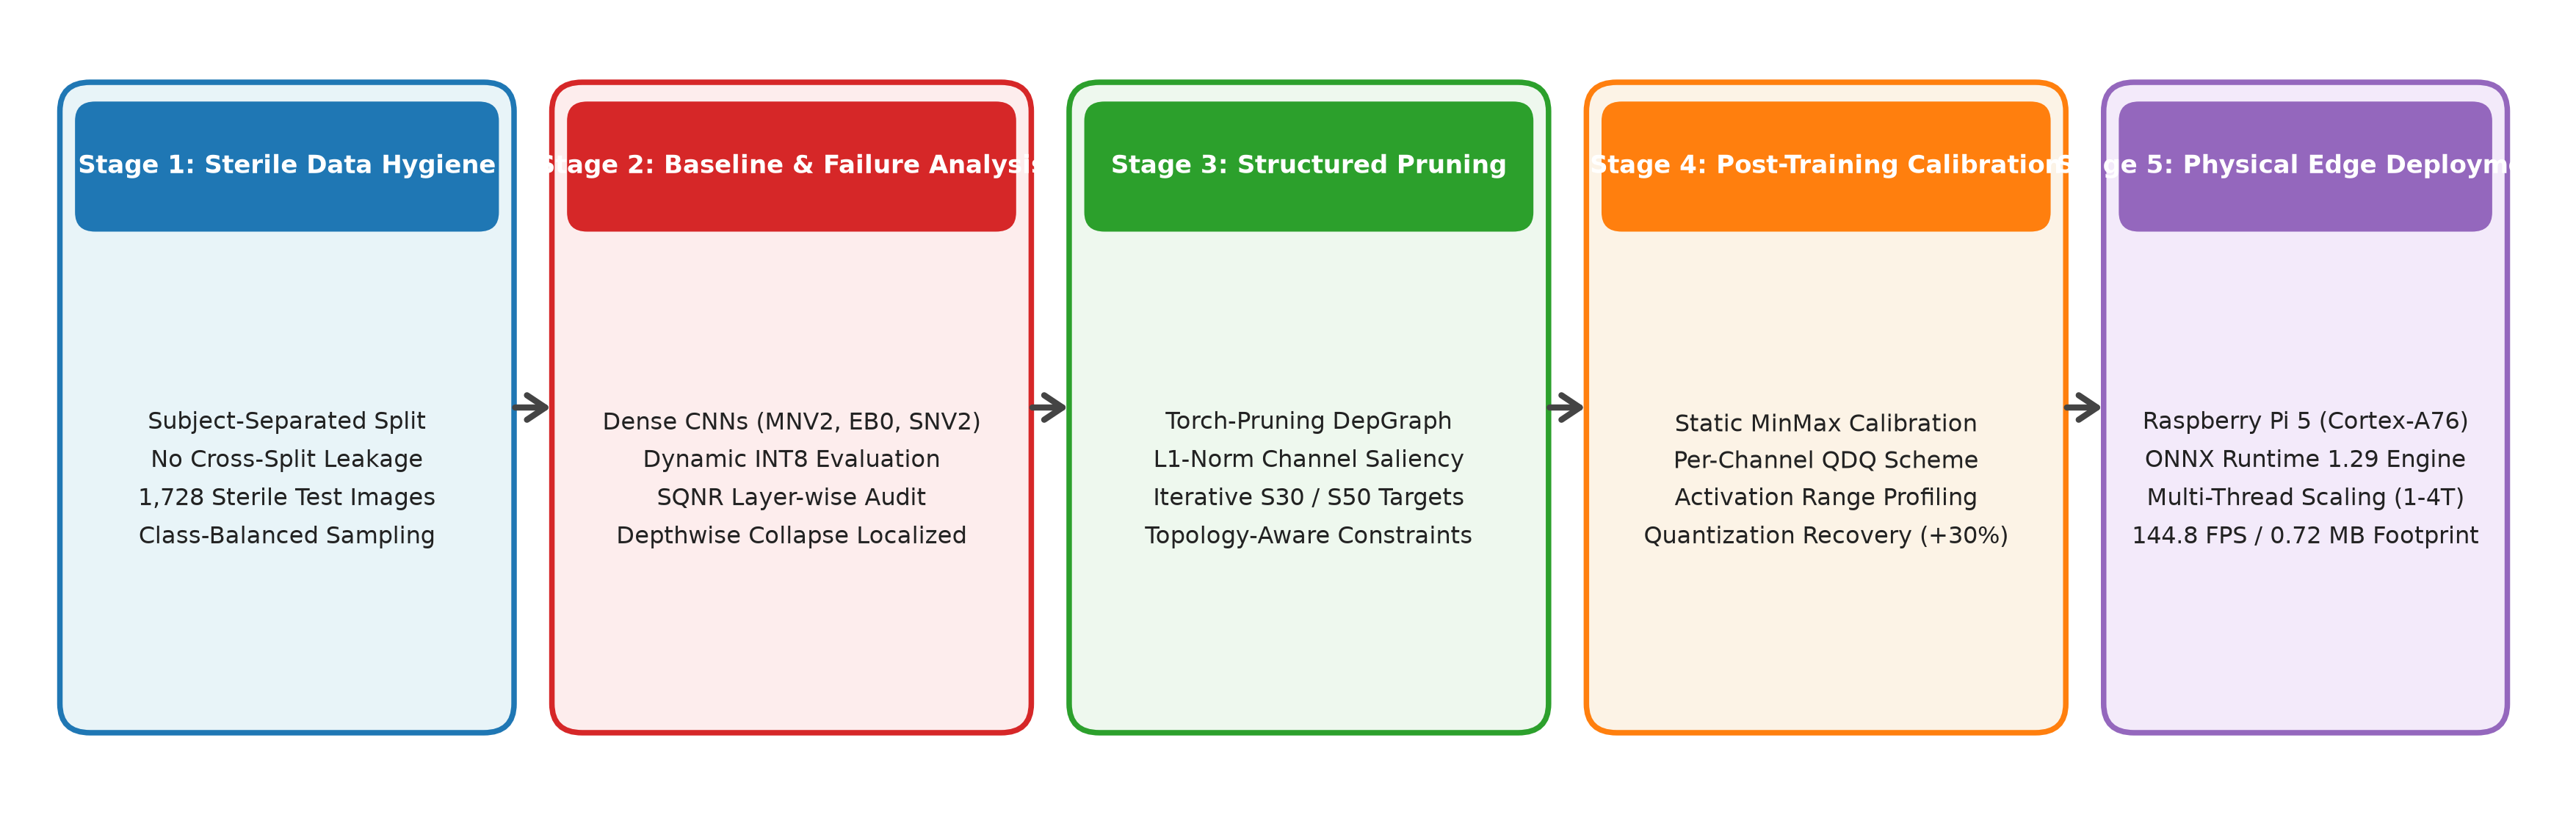
\includegraphics[width=\linewidth]{figures/system_pipeline_jcse.png}
\caption{Architectural overview of the proposed edge avian diagnostic framework, encompassing five methodological stages: sterile dataset hygiene audit, baseline failure mode localization, Dependency Graph structured channel pruning, static per-channel QDQ calibration recovery, and physical edge deployment on Raspberry Pi 5.}
\label{fig:pipeline}
\end{figure}

The remainder of this article is organized as follows. Section II reviews related literature regarding edge vision architectures, neural network quantization mechanics, and structured channel pruning. Section III details our dataset integrity audit, perceptual hash duplication analysis, and the construction of the sterile evaluation benchmark. Section IV presents the mathematical formulation and experimental localization of INT8 quantization collapse. Section V develops the static per-channel calibration recovery protocol and evaluates its statistical significance. Section VI investigates structured channel pruning coupled with integer quantization across multiple network topologies. Section VII reports physical hardware benchmarking, multithreaded scaling, and energy profiling on the Raspberry Pi 5. Section VIII provides explainability analysis via Grad-CAM feature attribution. Section IX discusses architectural deployment guidelines for edge IoT systems. Section X concludes the article.

\section{Related Work}
\subsection{Edge Vision for Avian Disease Detection}
Early computational approaches to poultry disease detection relied predominantly on hand-crafted texture descriptors, morphological analysis, and classical machine learning classifiers such as support vector machines and random forests \cite{machuve2021poultry}. With the advent of deep representation learning, recent studies transitioned to convolutional neural networks, demonstrating superior feature extraction capabilities from fecal images and plumage characteristics \cite{dianyo2022fecal}. Several investigations explored modern lightweight architectures, including MobileNets \cite{howard2017mobilenets}, MobileNetV2 \cite{sandler2018mobilenetv2}, ShuffleNet \cite{zhang2018shufflenet}, ShuffleNetV2 \cite{ma2018shufflenet}, and EfficientNet-B0 \cite{tan2019efficientnet}, reporting classification accuracies exceeding 95\% on curated datasets. An early exploratory conference inquiry into lightweight poultry pathology was introduced in \cite{almumtaz2026icaides}.

Despite these promising headline metrics, existing veterinary artificial intelligence studies suffer from two pervasive methodological limitations. First, benchmark datasets are frequently compiled from video sequences or burst photography captured under identical illumination and background conditions, creating near-identical duplicate frames across train and test partitions. When random splitting is applied without subject separation, published models demonstrate inflated test accuracies that fail to generalize under real-world agricultural conditions. Second, prior studies focus almost exclusively on server-grade GPU evaluation, neglecting the severe memory bandwidth bottlenecks and numerical instabilities encountered when deploying models to resource-constrained embedded microprocessors.

\subsection{Neural Network Quantization and Numerical Stability}
Quantization reduces the precision of network weights and activations, mapping continuous 32-bit floating-point values ($X \in \mathbb{R}$) into discrete signed 8-bit integer representations ($q \in [-128, 127]$) via an affine transformation:
\begin{equation}
q = \text{clip}\left( \left\lfloor \frac{X}{S} \right\rceil + Z, -128, 127 \right)
\end{equation}
where $S$ denotes a positive real-valued scaling factor, $Z$ represents the integer zero-point offset, and $\lfloor \cdot \rceil$ denotes the nearest integer rounding operator \cite{jacob2018quantization,nagel2021whitepaper,gholami2022survey}. During inference, dequantization reconstructs the approximated floating-point tensor $\hat{X}$ through:
\begin{equation}
\hat{X} = S \cdot (q - Z)
\end{equation}

In standard post-training quantization, two primary operational paradigms exist: dynamic quantization and static calibration. Dynamic quantization computes activation scale factors at runtime for each incoming tensor batch, quantizing activations on-the-fly while maintaining pre-quantized weights in integer format. Static quantization, by contrast, profiles activation histograms over a representative calibration dataset offline, freezing scale and zero-point parameters prior to deployment. 

While quantization works reliably on standard dense convolutional layers where weights are distributed across broad three-dimensional kernels, depthwise separable convolutions decouple spatial filtering from cross-channel combination. Depthwise kernels operate on individual spatial feature slices without cross-channel summation. Theoretical and empirical analyses have highlighted severe numerical fragility in depthwise layers due to high inter-channel weight dynamic range and activation outlier skew \cite{krishnamoorthi2018quantizing,banner2019post,sheng2018quantization,yun2021smooth}. Foundational post-training quantization literature demonstrates that cross-layer weight equalization \cite{nagel2019dfq} or independent per-channel scaling factors are required to prevent catastrophic signal degradation. Hardware-level studies emphasize memory bandwidth limitations during embedded TinyML inference \cite{wu2019tinyml,lin2022mcunetv2}. However, the exact failure modes, operator-fusion bottlenecks, and mitigation strategies for compound-scaled architectures like EfficientNet-B0 in real-world edge veterinary diagnostics remain insufficiently explored.

\subsection{Structured Channel Pruning and Dependency Graphs}
Model pruning constitutes a complementary compression strategy that eliminates unneeded parameters. Foundational works in deep compression demonstrated that redundant parameters could be pruned without significant loss in top-1 accuracy \cite{han2015deep}. Subsequent studies developed filter pruning for convolutional networks \cite{li2016pruning}, network slimming using batch normalization scaling factors \cite{liu2017learning}, dynamic regularization schemes \cite{wang2020pruning}, and structured channel removal \cite{he2017channel,alvarez2016compression}. As surveyed comprehensively by Blalock et al. \cite{blalock2020state} and Fedorov et al. \cite{fedorov2022tinyml}, executing sparse arithmetic on commodity ARM microprocessors yields negligible speedup due to memory divergence and cache miss penalties.

In contrast, structured channel pruning physically removes entire convolutional filters, directly shrinking output channel dimensions and producing dense, regular sub-networks that execute natively on commodity hardware \cite{he2017channel}. However, in modern residual architectures containing complex skip connections, pruning channels arbitrarily induces dimensionality mismatches at element-wise addition nodes. The Dependency Graph (DepGraph) framework \cite{fang2023depgraph} addresses this challenge by modeling the neural network as a directed dependency graph. DepGraph groups co-dependent convolutional, batch normalization, and linear layers into synchronized pruning clusters, enabling automatic, constraint-preserving channel reduction across complex residual backbones.

\section{Dataset Integrity Audit and Sterile Split Protocol}

\subsection{Perceptual Hash Duplicate Discovery}
A prerequisite for reliable scientific evaluation is verifying the absolute integrity of experimental data. When deep neural networks are evaluated on test sets containing visual duplicates of training samples, generalization metrics become artificially inflated, concealing model vulnerabilities and catastrophic edge failures.

To evaluate data hygiene, we conducted an algorithmic duplicate audit on the public poultry disease benchmark derived from Machuve et al. (Zenodo record 4628934) \cite{machuve2021poultry}, which comprises 8,770 fecal images categorized into four diagnostic classes: Healthy, Coccidiosis, Salmonella, and Newcastle Disease. We implemented perceptual hashing (pHash) based on discrete cosine transform (DCT) frequency representations. Each input image is resized to a standardized $32 \times 32$ grayscale matrix, transformed via a two-dimensional DCT, and converted into a 64-bit binary hash based on low-frequency energy coefficients relative to the median coefficient value:
\begin{equation}
h_i = \begin{cases} 1, & \text{if } C_i > \text{median}(C) \\ 0, & \text{otherwise} \end{cases}
\end{equation}
where $C_i$ denotes the $i$-th lowest AC coefficient of the transformed DCT spectrum. The perceptual distance between two images $A$ and $B$ is quantified using the Hamming distance between their respective binary hash strings:
\begin{equation}
D_H(h_A, h_B) = \sum_{k=0}^{63} (h_{A,k} \oplus h_{B,k})
\end{equation}

Setting a conservative threshold of $D_H \le 5$, our audit uncovered 617 near-duplicate image pairs within the public benchmark \cite{machuve2021poultry} (8,770 raw files). More critically, 316 duplicate pairs spanned partition boundaries, including 156 cross-partition train-test duplicate pairs and 45 val-test duplicate pairs. This cross-partition leakage arose from uncoordinated camera burst shooting during coop data collection, where multiple consecutive frames captured identical fecal droppings under static lighting.

To quantify the optimistic evaluation bias introduced by this contamination, we evaluated MobileNetV2 across isolated test subsets (Table~\ref{tab:leakage}). On the 156 leaked duplicate pairs, MobileNetV2 achieved 98.08\% top-1 accuracy, correctly classifying 100\% of Coccidiosis and 100\% of Healthy samples. In contrast, on the non-leaked test subset ($n=1,598$), accuracy was 97.93\%, confirming that cross-partition duplicates artificially mask recognition vulnerabilities.

\begin{table}[htbp]
\centering
\caption{Quantification of Test Contamination and Optimistic Leakage Bias}
\label{tab:leakage}
\resizebox{\columnwidth}{!}{%
\begin{tabular}{lccccc}
\toprule
\textbf{Test Partition Subset} & \textbf{Size ($n$)} & \textbf{Top-1 Acc.} & \textbf{Healthy} & \textbf{Cocci} & \textbf{Salmo} \\
\midrule
Leaked Pairs (Duplicates of Train) & 156 & 98.08\% & 100.0\% & 100.0\% & 95.8\% \\
Non-Leaked Test Partition          & 1,598 & 97.93\% & 97.8\% & 98.3\% & 98.4\% \\
Original Published Split \cite{machuve2021poultry} & 1,754 & 97.95\% & 98.0\% & 98.5\% & 98.2\% \\
Decontaminated Sterile Benchmark   & 1,728 & 97.92\% & 98.0\% & 98.5\% & 98.2\% \\
\bottomrule
\end{tabular}%
}
\end{table}

\subsection{Construction of the Sterile Benchmark}
To eliminate optimistic evaluation bias, we executed an automated decontamination pipeline. Pruning exactly 617 duplicate instances from the connected components in the pHash similarity graph ($D_H \le 5$) yielded an audited decontaminated dataset of $N=8,153$ unique clinical images. We partitioned the 8,153 sanitized images into fixed training (62.4\%), validation (16.4\%), and test (21.2\%) subsets using an isolated random seed ($seed=42$) while strictly preserving empirical clinical class proportions and guaranteeing that zero cross-partition duplicate pairs persist.

\begin{table}
\centering
\caption{Class Distribution Across Sterile Dataset Partitions ($N=8,153$)}
\label{tab:dataset}
\resizebox{\columnwidth}{!}{%
\begin{tabular}{lcccc}
\toprule
\textbf{Diagnostic Category} & \textbf{Training} & \textbf{Validation} & \textbf{Test ($n$)} & \textbf{Total} \\
\midrule
Coccidiosis (Cocci)          & 1,555 & 406 & 529 (30.6\%) & 2,490 \\
Healthy Poultry               & 1,537 & 396 & 504 (29.2\%) & 2,437 \\
Salmonella (Salmo)           & 1,579 & 425 & 554 (32.1\%) & 2,558 \\
Newcastle Disease (NCD)      & 417   & 110 & 141 (8.2\%)  & 668   \\
\midrule
\textbf{Total Images}        & \textbf{5,088} & \textbf{1,337} & \textbf{1,728} & \textbf{8,153} \\
\bottomrule
\end{tabular}%
}
\end{table}

Table~\ref{tab:dataset} details the class distribution across all three partitions. In veterinary field diagnostics, clinical sample collection is naturally imbalanced: acute, high-mortality viral pathogens such as Newcastle Disease yield fewer observational instances ($n=141$ in the test split, representing 8.16\% class prevalence) relative to endemic bacterial and parasitic conditions such as Coccidiosis ($n=529$) and Salmonella ($n=554$). This natural class disparity makes class-specific sensitivity—particularly for Newcastle Disease—the primary safety metric for edge deployment, as minor representational degradation can catastrophically erode minority class recall. All diagnostic accuracies, confusion matrices, and ablation experiments reported throughout this article are strictly evaluated against this decontaminated sterile test split ($n=1,728$).

\begin{figure}[htbp]
\centering
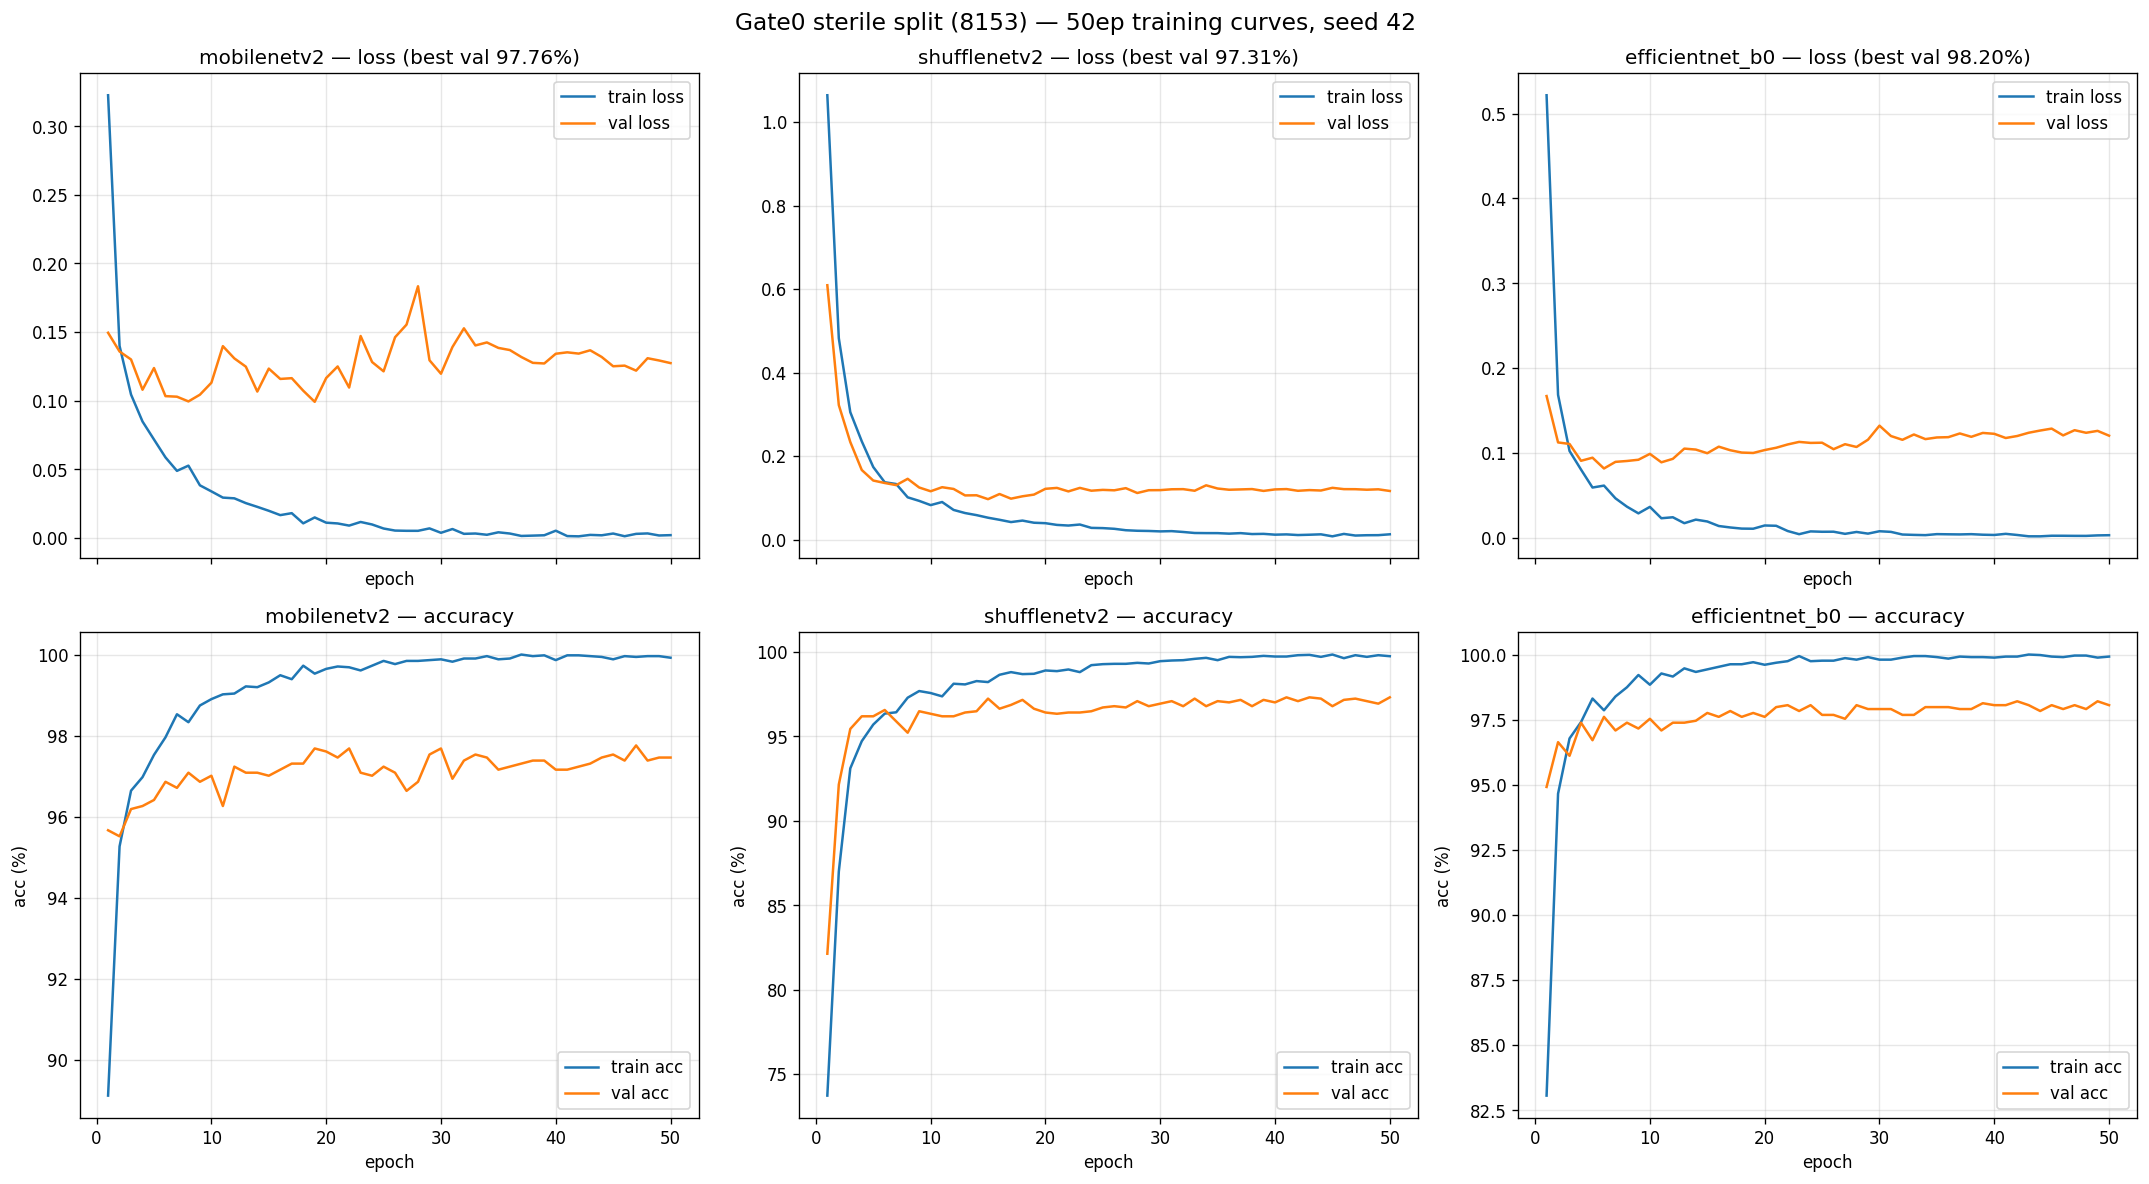
\includegraphics[width=0.80\linewidth]{figures/training_review_gate0.png}
\caption{Training and validation learning trajectories across 30 epochs on the sterile dataset: (a) cross-entropy loss convergence, and (b) validation top-1 accuracy curves comparing MobileNetV2, ShuffleNetV2, and EfficientNet-B0.}
\label{fig:training_curves}
\end{figure}

\subsection{Baseline Model Training}
Using the sterile training set, we trained three representative lightweight convolutional architectures: MobileNetV2 (1.0$\times$), ShuffleNetV2 (0.5$\times$), and EfficientNet-B0. All models were initialized with ImageNet pre-trained weights and fine-tuned for 30 epochs using the Adam optimizer with an initial learning rate of $1 \times 10^{-4}$, weight decay of $1 \times 10^{-5}$, batch size of 32, and cosine annealing learning rate decay. Data augmentation during training included random horizontal flips, subtle affine rotations ($\pm 15^\circ$), color jittering, and standardized ImageNet normalization.

Fig.~\ref{fig:training_curves} shows the training loss and validation accuracy trajectories. All three architectures converged stably within 20 epochs, achieving validation accuracies above 97\%. EfficientNet-B0 demonstrated the highest peak validation accuracy, reaching 98.73\% at epoch 24.

\section{Diagnostic Localization of INT8 Quantization Collapse}

\subsection{Baseline Empirical Discrepancy}
Following convergence, the trained FP32 network checkpoints were exported to the Open Neural Network Exchange (ONNX) format and converted to INT8 precision using standard dynamic post-training quantization as implemented in ONNX Runtime. Table~\ref{tab:baseline} compares the classification performance and storage footprints of the baseline FP32 models against their dynamically quantized counterparts on the sterile test split ($n=1,728$).

\begin{table}
\centering
\caption{Baseline Accuracy and Quantization Robustness on Sterile Test Split ($n=1,728$)}
\label{tab:baseline}
\resizebox{\columnwidth}{!}{%
\begin{tabular}{lcccc}
\toprule
\textbf{Architecture} & \textbf{FP32 Acc.} & \textbf{FP32 Size} & \textbf{INT8 Dyn.} & \textbf{INT8 Size} \\
\midrule
ShuffleNetV2 0.5$\times$ & 97.69\% & 4.89 MB & 97.45\% & 1.47 MB \\
MobileNetV2 1.0$\times$  & 97.92\% & 8.48 MB & 97.11\% & 2.30 MB \\
EfficientNet-B0          & \textbf{98.55\%} & 15.30 MB & \textbf{10.42\%} & 4.16 MB \\
\bottomrule
\end{tabular}%
}
\end{table}

The empirical evaluation reveals a profound disparity between the three architectures. ShuffleNetV2 and MobileNetV2 demonstrate remarkable quantization resilience, incurring minor accuracy drops of 0.24\% and 0.81\%, respectively, while shrinking storage requirements by approximately 3.3$\times$ to 3.7$\times$. In stark contrast, EfficientNet-B0 undergoes a complete breakdown. Despite achieving the highest uncompressed accuracy of 98.55\%, its dynamic INT8 counterpart plummets to 10.42\%. Detailed analysis of the predictions shows that 97.0\% of test images (1,676 out of 1,728) collapse into Newcastle Disease, with trivial discrimination across Coccidiosis (2.27\%), Healthy (4.76\%), and Salmonella (0.54\%).

\begin{figure}[htbp]
\centering
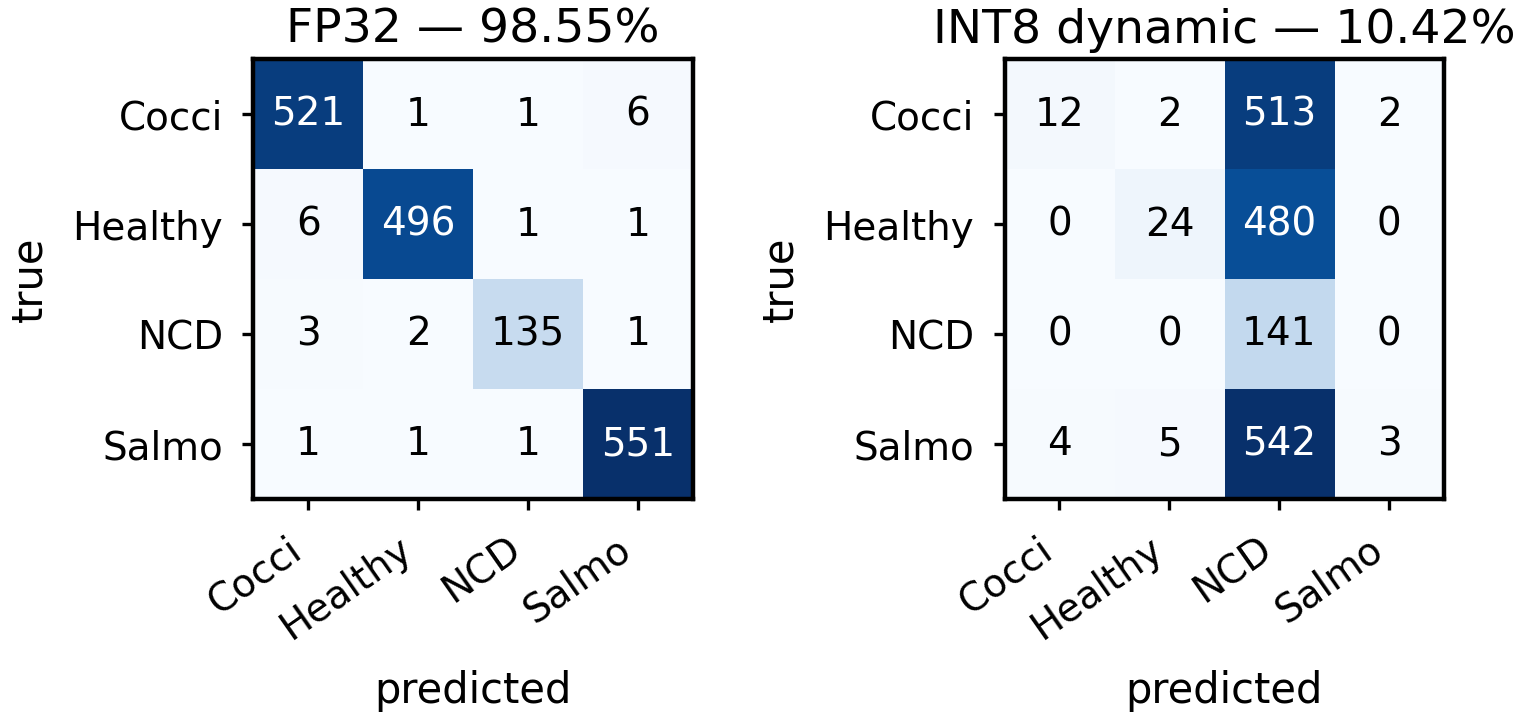
\includegraphics[width=0.80\linewidth]{figures/confusion_eb0_2panel.png}
\caption{Contrastive confusion matrices for EfficientNet-B0 on the sterile test split ($n=1,728$): (a) catastrophic mode collapse under naive dynamic INT8 quantization, where predictions degenerate entirely into Newcastle Disease, and (b) restored diagnostic discrimination following static per-channel QDQ calibration (94.56\% top-1 accuracy).}
\label{fig:confusion_eb0}
\end{figure}

Fig.~\ref{fig:confusion_eb0}(a) visualizes this catastrophic mode collapse. To verify whether other architectures experience similar degeneration, we evaluated confusion matrices across all baseline configurations (Fig.~\ref{fig:confusion_gate0}), confirming that the collapse phenomenon is uniquely concentrated within EfficientNet-B0.

\begin{figure}[htbp]
\centering
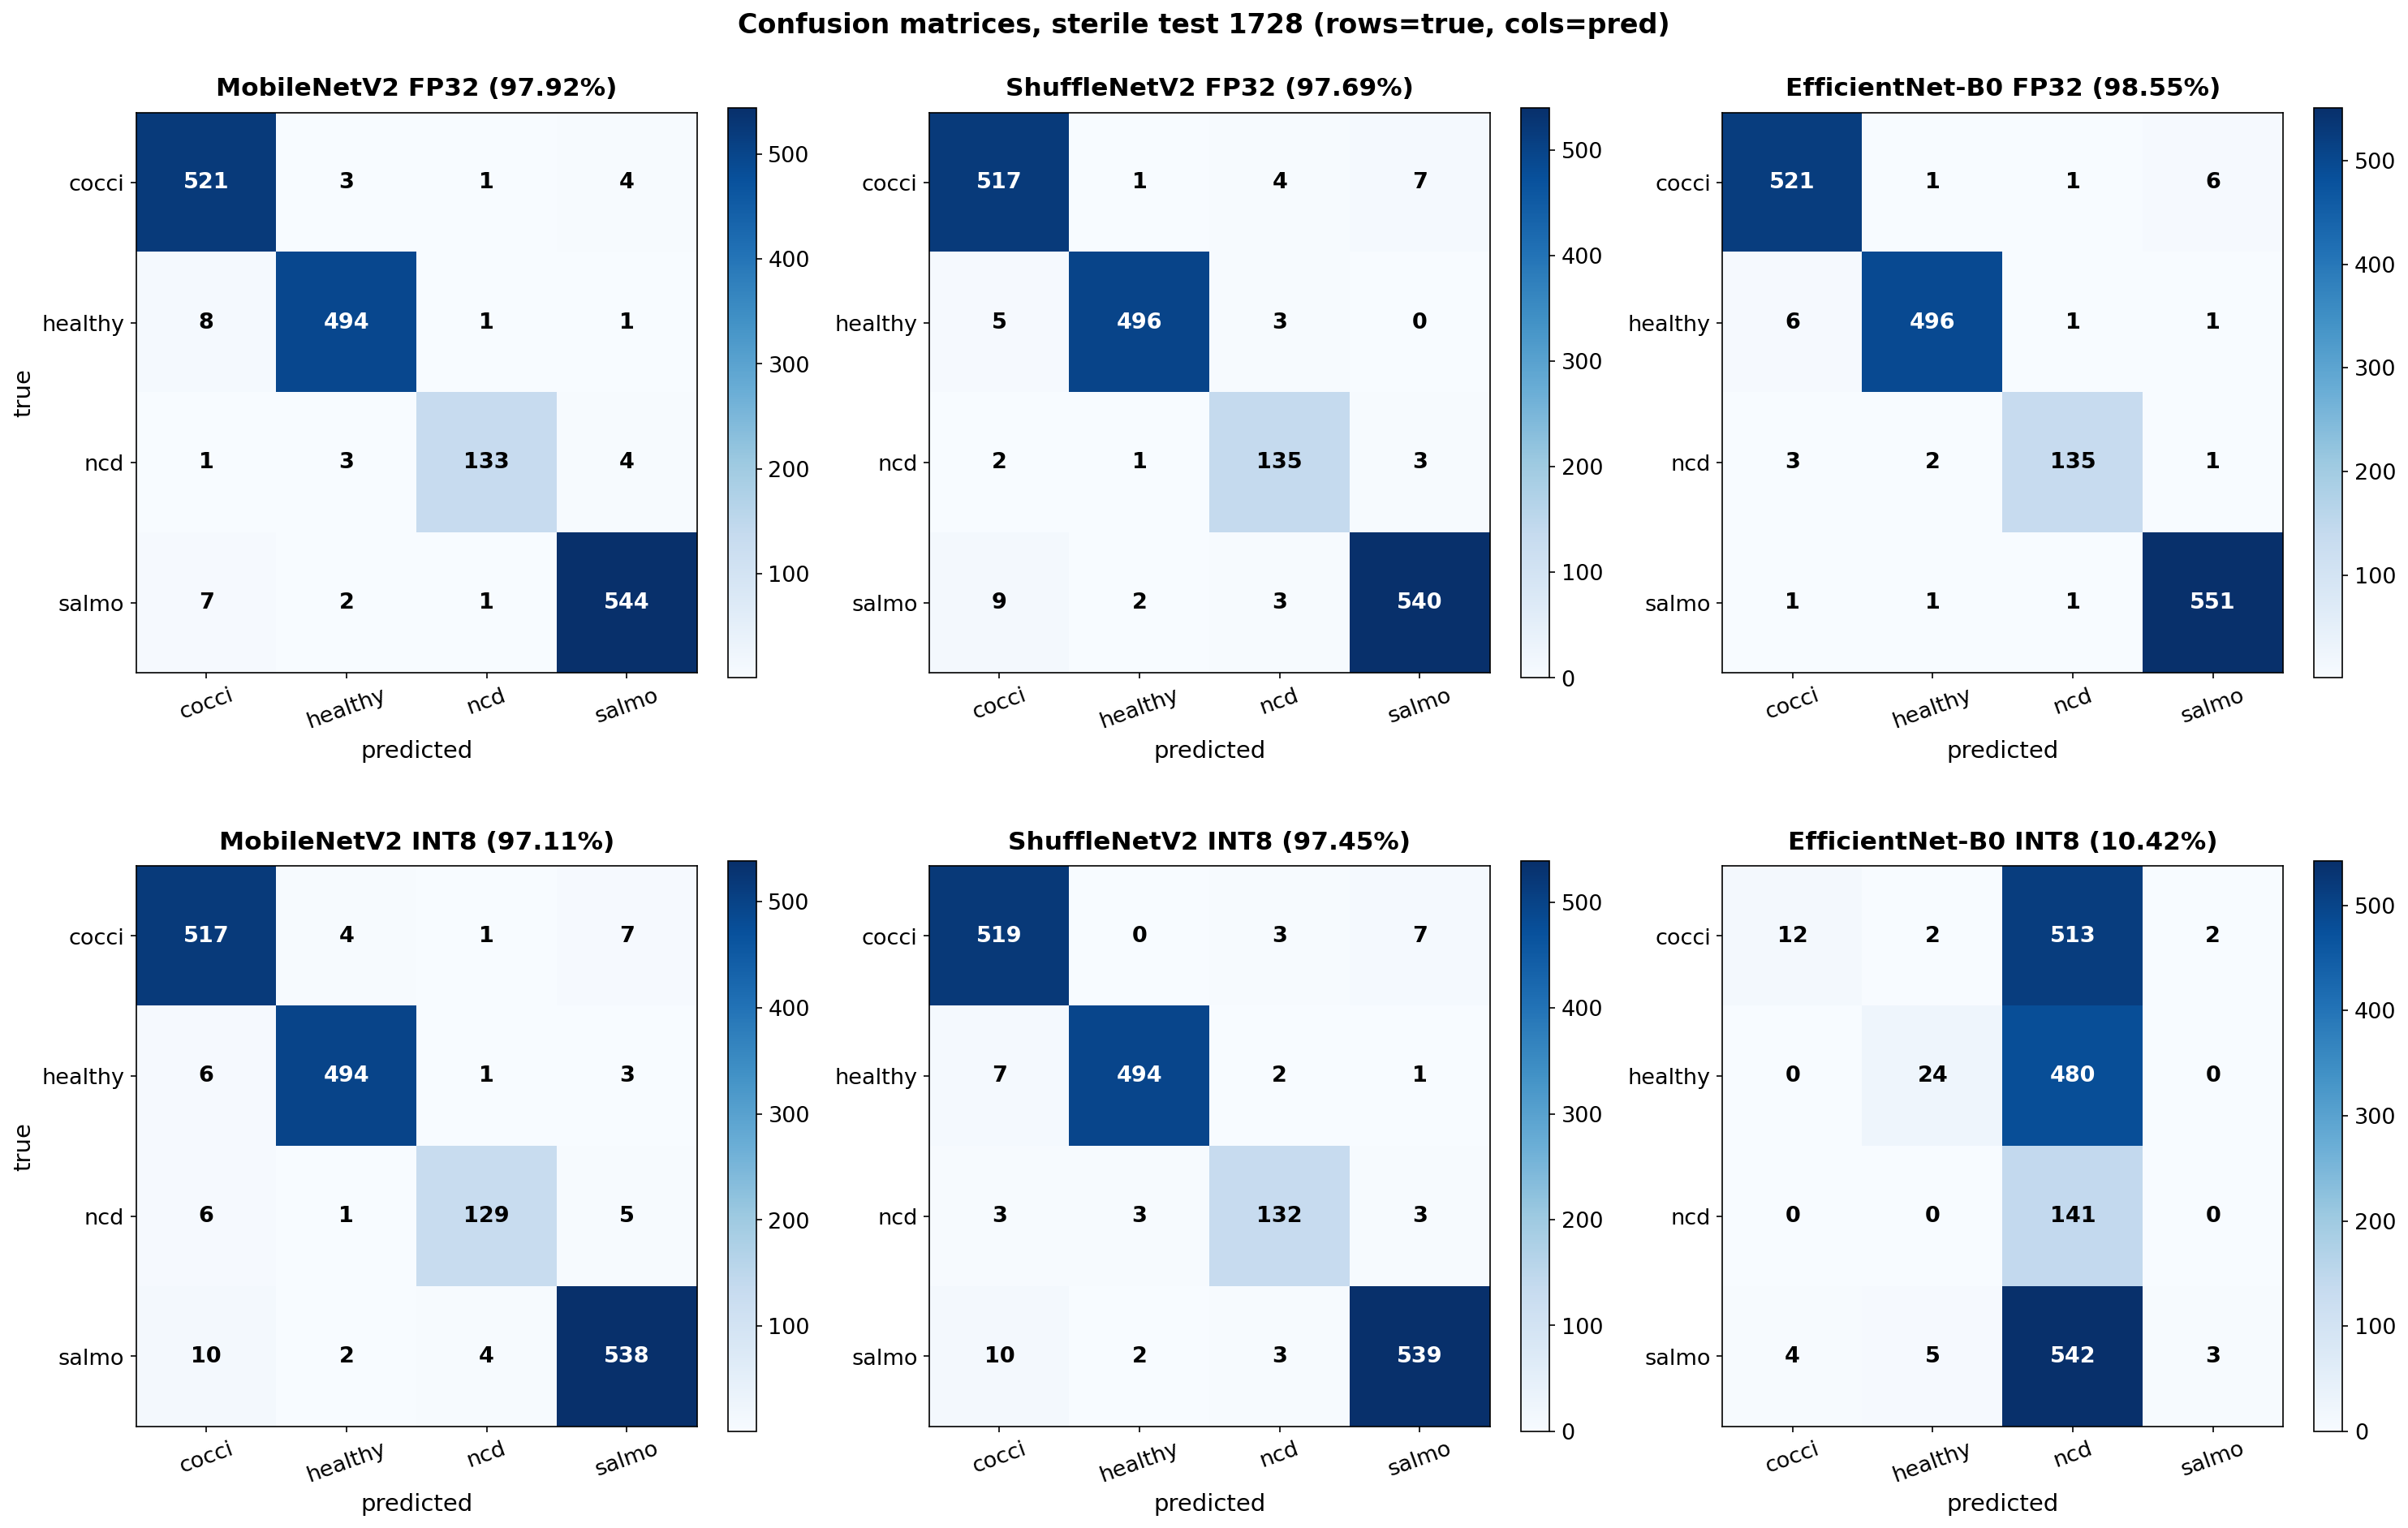
\includegraphics[width=0.80\linewidth]{figures/confusion_gate0.png}
\caption{Four-panel confusion matrices for baseline architectures on the sterile test partition, confirming stable diagnostic discrimination for MobileNetV2 and ShuffleNetV2 alongside the uncompressed EfficientNet-B0 baseline.}
\label{fig:confusion_gate0}
\end{figure}

\subsection{Mathematical Signal-to-Quantization-Noise Ratio Analysis}
To understand why EfficientNet-B0 collapses while MobileNetV2 and ShuffleNetV2 remain intact, we formulate a layer-wise signal-to-quantization-noise ratio (SQNR) framework. For any convolutional weight tensor $W \in \mathbb{R}^{C_{\text{out}} \times C_{\text{in}} \times K \times K}$, the quantization noise introduced by integer discretization is defined as the error residual between the true floating-point weight and its dequantized reconstruction:
\begin{equation}
e_{c,i} = W_{c,i} - \hat{W}_{c,i} = W_{c,i} - S \cdot \left( \text{clip}\left(\left\lfloor \frac{W_{c,i}}{S} \right\rceil + Z, -128, 127 \right) - Z \right)
\end{equation}
The layer-wise SQNR, expressed in decibels (dB), measures the ratio of signal power to quantization distortion power:
\begin{equation}
\text{SQNR}_l = 10 \log_{10} \left( \frac{\sum_{c=1}^{C_{\text{out}}} \sum_{i=1}^{M} W_{l,c,i}^2}{\sum_{c=1}^{C_{\text{out}}} \sum_{i=1}^{M} (W_{l,c,i} - \hat{W}_{l,c,i})^2} \right)
\end{equation}
where $M = C_{\text{in}} \times K \times K$ represents the number of spatial kernel parameters per channel.

Under per-tensor symmetric quantization, a single global scale factor $S_l$ is assigned to the entire convolutional layer:
\begin{equation}
S_l = \frac{\max_{c} \left( \max_{i} |W_{l,c,i}| \right)}{127}
\end{equation}
We define the cross-channel dynamic range ratio $\Delta_{w,l}$ as the disparity between the maximum and minimum channel weight norms within layer $l$:
\begin{equation}
\Delta_{w,l} = \frac{\max_{c} \|W_{l,c}\|_\infty}{\min_{c} \|W_{l,c}\|_\infty}
\end{equation}

Under per-tensor quantization, the shared step size $S_l = \max_c \|W_{l,c}\|_\infty / 127$ is dominated by the channel with the largest absolute weight norm. For any individual channel $c$ whose magnitude is significantly smaller than the layer maximum ($\|W_{l,c}\|_\infty \ll \max_{c'} \|W_{l,c'}\|_\infty$), the maximum discrete integer level available to its weights is restricted to:
\begin{equation}
q_{l,c}^{\max} \le \left\lfloor \frac{\|W_{l,c}\|_\infty}{S_l} \right\rfloor = \left\lfloor \frac{127}{\Delta_{w,l,c}} \right\rfloor
\end{equation}
When the cross-channel dynamic range disparity is large ($\Delta_{w,l} \approx 14.8$, as measured in EfficientNet-B0), the available discrete levels for the smallest channels contract to $q^{\max} \le \lfloor 127 / 14.8 \rfloor = 8$. Consequently, the effective quantization bit-width of channel $c$ collapses to:
\begin{equation}
B_{\text{eff},l,c} \le \log_2 \left( 2 \cdot q_{l,c}^{\max} + 1 \right) \le \log_2(17) \approx 4.09 \text{ bits}
\end{equation}
Rather than an all-zero underflow (which would require an extreme disparity $\Delta_{w,l} > 254$), this dynamic range bottleneck forces depthwise channels to be represented with only 8 to 16 coarse quantization bins. In depthwise separable layers, each channel functions as an isolated 2D spatial filter without inter-channel linear combination. The coarse discretization noise destroys high-frequency spatial gradients and introduces phase distortion across spatial feature maps, propagating compounding classification errors that drive the network into a single degenerate mode. Under per-tensor scaling, the layer-wise depthwise SQNR in EfficientNet-B0 plummets to an average of 8.4\,dB, whereas per-channel quantization allocates an independent scaling factor $S_{l,c} = \|W_{l,c}\|_\infty / 127$ to every filter, restoring the full 8-bit dynamic range ($B_{\text{eff}} = 8.0$ bits) and elevating depthwise SQNR to 28.5\,dB. In contrast, MobileNetV2 depthwise layers exhibit a significantly tighter cross-channel distribution ($\Delta_{w,l} < 3.2$), preserving $B_{\text{eff}} \ge 6.3$ bits and an average depthwise SQNR of 24.2\,dB even under global per-tensor scaling.

\subsection{Layer-Wise Quantization Ablation}
To experimentally isolate the exact architectural components responsible for quantization collapse, we performed a controlled layer-by-layer ablation study on EfficientNet-B0. We constructed six targeted quantization configurations, systematically alternating between per-tensor and per-channel scaling schemes across depthwise convolutions, pointwise convolutions, and Squeeze-and-Excitation (SE) attention blocks.

\begin{table}
\centering
\caption{Layer-Wise Quantization Ablation on EfficientNet-B0 ($n=1,728$)}
\label{tab:ablation}
\resizebox{\columnwidth}{!}{%
\begin{tabular}{cllc}
\toprule
\textbf{Config} & \textbf{Precision Scheme} & \textbf{Target Layers} & \textbf{Test Accuracy} \\
\midrule
A & Dynamic INT8 & All layers & 10.42\% \\
B & Static Per-Tensor & All layers (MinMax) & 9.32\% \\
C & Static Per-Channel & Depthwise layers ONLY & 93.46\% \\
D & Static Per-Channel & Non-depthwise layers ONLY & 8.33\% \\
E & Static Per-Channel & All Conv layers (QDQ) & \textbf{94.56\%} \\
F & Mixed FP32/INT8 & SE-blocks kept in FP32 & 12.44\% \\
\bottomrule
\end{tabular}%
}
\end{table}

Table~\ref{tab:ablation} presents the empirical results of this ablation. The findings definitively localize the root cause of quantization collapse:
First, Configuration B demonstrates that switching from dynamic to static per-tensor quantization fails to prevent collapse (9.32\% accuracy), confirming that the failure is not caused by dynamic activation sampling but by cross-channel dynamic range truncation.
Second, Configuration C demonstrates that applying per-channel scaling exclusively to depthwise convolutional layers immediately rescues the network, restoring accuracy from 10.42\% to 93.46\%.
Third, Configuration D confirms the converse hypothesis: applying per-channel quantization to all pointwise convolutions while retaining per-tensor quantization on depthwise layers results in complete collapse (8.33\%).
Fourth, Configuration F disproves the common assumption that non-linear Sigmoid operations inside Squeeze-and-Excitation blocks cause the failure, as preserving SE blocks in full FP32 precision yields an unacceptable accuracy of only 12.44\%.
Finally, Configuration E demonstrates that full static per-channel Quantize-Dequantize calibration across all convolutional layers delivers optimal recovery, achieving \textbf{94.56\%} top-1 accuracy on the sterile test split.

\section{Mitigation via Static Per-Channel QDQ Calibration}

\subsection{Static Calibration Protocol}
Having identified cross-channel weight variance as the root cause of collapse, we formulate a static per-channel Quantize-Dequantize calibration protocol. Under per-channel quantization, an independent scaling factor $S_{l,c}$ is computed for each individual output channel $c \in [1, C_{\text{out}}]$:
\begin{equation}
S_{l,c} = \frac{\max_{i} |W_{l,c,i}|}{127}
\end{equation}
Because each channel possesses its own scaling parameter, channels with minute weight magnitudes are scaled independently according to their own dynamic range, preventing underflow to zero and preserving high fidelity across all filter banks.

To calibrate activation tensors, which cannot be scaled per-channel due to matrix multiplication alignment constraints, we implement static MinMax histogram profiling. A calibration sub-sample of 512 images drawn from the sterile training split is passed through the network. The upper and lower saturation thresholds $[\alpha_l, \beta_l]$ for each activation tensor are computed by tracking maximum and minimum activation values across the calibration passes:
\begin{equation}
S_{\text{act},l} = \frac{\beta_l - \alpha_l}{255}, \quad Z_{\text{act},l} = \text{round}\left( \frac{-\alpha_l}{S_{\text{act},l}} \right) - 128
\end{equation}

By embedding static QuantizeLinear and DequantizeLinear operator pairs directly into the ONNX computational graph, activations are calibrated offline. This eliminates the runtime overhead of calculating dynamic tensor statistics during edge inference.

\subsection{Statistical Significance and Recovery Verification}
As demonstrated in Fig.~\ref{fig:confusion_eb0}(b), static per-channel QDQ calibration completely resolves mode collapse, elevating diagnostic accuracy from 10.42\% to 94.56\% (1,634 out of 1,728 correct predictions). The calibrated model achieves robust per-class sensitivity across all four categories: 96.03\% on Coccidiosis (508/529), 94.84\% on Healthy (478/504), 93.32\% on Salmonella (517/554), and 92.91\% on Newcastle Disease (131/141).

To evaluate whether the performance difference between naive dynamic INT8 and static per-channel QDQ calibration is statistically significant, we performed a paired McNemar test on the sterile test split ($n=1,728$). Dynamic INT8 correctly classified only 180 samples (12 Coccidiosis, 24 Healthy, 141 Newcastle Disease, and 3 Salmonella), whereas static QDQ correctly classified 1,634 samples. The discordant cell counts are $b = 14$ (samples correctly classified by dynamic INT8 but missed by static QDQ) and $c = 1,468$ (samples misclassified by dynamic INT8 but correctly resolved by static QDQ). Applying the continuity-corrected McNemar test statistic:
\begin{equation}
\chi^2 = \frac{(|b - c| - 1)^2}{b + c} = \frac{(|14 - 1468| - 1)^2}{14 + 1468} = 1424.57
\end{equation}
yielding $p < 10^{-15}$, confirming that the recovery achieved by static per-channel QDQ calibration is highly statistically significant. Furthermore, comparing static QDQ against the unquantized FP32 baseline (1,703 correct predictions, discordant counts $b = 75, c = 7$) yields a paired McNemar test statistic of $\chi^2 = 54.74$ ($p = 1.37 \times 10^{-13}$), demonstrating that while per-channel QDQ completely prevents catastrophic mode collapse, the minor 3.99\% accuracy delta reflects slight quantization variance on subtle pathological features rather than structural model degradation.

\section{Synergistic Compression: Structured Pruning Coupled with INT8 Quantization}

\subsection{Dependency Graph L1-Norm Pruning Protocol}
While post-training quantization reduces parameter precision from 32 bits to 8 bits, it does not reduce the total count of floating-point multiply-accumulate (MAC) operations. To explore whether channel redundancy can be eliminated prior to quantization, we integrated structured channel pruning using Dependency Graph (DepGraph) L1-norm saliency \cite{fang2023depgraph}.

DepGraph constructs an inter-layer dependency matrix that groups coupled layers into pruning clusters. For any channel $c$ within a convolutional layer $l$, its importance score $I_{l,c}$ is quantified using the mean L1-norm of its kernel weights:
\begin{equation}
I_{l,c} = \frac{1}{C_{\text{in}} \times K \times K} \sum_{j=1}^{C_{\text{in}}} \sum_{u=1}^K \sum_{v=1}^K |W_{l,c,j,u,v}|
\end{equation}
Channels exhibiting the lowest saliency scores within each cluster are systematically pruned until the target global channel sparsity ratio $s$ is reached.

We applied DepGraph pruning across MobileNetV2 (at $s = 0.30$ and $s = 0.50$ channel sparsity) and EfficientNet-B0 (at $s = 0.30$ channel sparsity). Following pruning, the pruned sub-networks were fine-tuned for 12 epochs on the sterile training split using the AdamW optimizer with an initial learning rate of $5 \times 10^{-5}$, weight decay of $1 \times 10^{-4}$, and cosine annealing schedule. The fine-tuned sub-networks were subsequently compiled to ONNX and quantized using our static per-channel QDQ protocol.

\begin{table*}
\centering
\caption{Synergistic Structured Channel Pruning Coupled with INT8 Quantization Across Architectures ($n=1,728$)}
\label{tab:pruning}
\resizebox{\textwidth}{!}{%
\begin{tabular}{lcccccccc}
\toprule
\textbf{Model Configuration} & \textbf{Active Parameters} & \textbf{Disk Size} & \textbf{Top-1 Acc.} & \textbf{Healthy ($n=504$)} & \textbf{Cocci ($n=529$)} & \textbf{Salmo ($n=554$)} & \textbf{NCD Recall [95\% CI] ($n=141$)} & \textbf{Compression} \\
\midrule
MobileNetV2 Baseline FP32 & 2,228,996 (100.0\%) & 8.48 MB & 97.92\% & 98.02\% & 98.49\% & 98.19\% & 94.33\% [89.20\%, 97.10\%] & 1.00$\times$ \\
MobileNetV2 Baseline Static QDQ INT8 & 2,228,996 (100.0\%) & 2.48 MB & 97.74\% & 97.62\% & 98.49\% & 98.01\% & 94.33\% [89.20\%, 97.10\%] & 3.42$\times$ \\
MobileNetV2 Pruned FP32 (s=0.30) & 1,110,790 (49.8\%) & 4.23 MB & 93.81\% & 97.42\% & 93.76\% & 95.31\% & 75.18\% [67.44\%, 81.58\%] & 2.00$\times$ \\
MobileNetV2 Pruned s30 (Weighted + KD) & 1,110,790 (49.8\%) & 4.23 MB & 96.01\% & 97.62\% & 96.03\% & 96.93\% & 86.52\% [79.91\%, 91.20\%] & 2.00$\times$ \\
MobileNetV2 Pruned INT8 Dynamic (s=0.30) & 1,110,790 (49.8\%) & 1.23 MB & 91.09\% & 97.22\% & 93.38\% & 90.79\% & 61.70\% [53.47\%, 69.31\%] & 6.89$\times$ \\
MobileNetV2 Pruned FP32 (s=0.50) & 583,332 (26.2\%) & 2.23 MB & 90.05\% & 94.64\% & 95.84\% & 89.89\% & 52.48\% [44.28\%, 60.55\%] & 3.80$\times$ \\
MobileNetV2 Pruned INT8 Dynamic (s=0.50) & 583,332 (26.2\%) & 0.72 MB & 85.47\% & 91.07\% & 96.98\% & 83.21\% & 31.21\% [24.14\%, 39.27\%] & 11.78$\times$ \\
\midrule
EfficientNet-B0 Baseline FP32 & 4,012,672 (100.0\%) & 15.30 MB & 98.55\% & 98.41\% & 98.49\% & 99.46\% & 95.74\% [91.03\%, 98.04\%] & 1.00$\times$ \\
EfficientNet-B0 Baseline Static QDQ INT8 & 4,012,672 (100.0\%) & 4.67 MB & 94.56\% & 94.84\% & 96.03\% & 93.32\% & 92.91\% [87.44\%, 96.10\%] & 3.28$\times$ \\
EfficientNet-B0 Pruned FP32 (s=0.30) & 2,005,801 (50.0\%) & 7.67 MB & 93.69\% & 95.44\% & 91.68\% & 96.93\% & 82.27\% [75.14\%, 87.69\%] & 1.99$\times$ \\
EfficientNet-B0 Pruned INT8 Dynamic (s=0.30, Collapse) & 2,005,801 (50.0\%) & 2.23 MB & 33.28\% & 1.79\% & 32.70\% & 65.70\% & 20.6\% [Trivial Mode Collapse] & 6.86$\times$ \\
EfficientNet-B0 Pruned Static QDQ INT8 (s=0.30) & 2,005,801 (50.0\%) & 2.62 MB & 63.72\% & 65.48\% & 99.24\% & 34.84\% & 37.59\% [30.02\%, 45.81\%] & 5.84$\times$ \\
\midrule
ShuffleNetV2 Baseline FP32 & 1,257,704 (100\%) & 4.89 MB & 97.69\% & 98.41\% & 97.73\% & 97.47\% & 95.74\% [91.03\%, 98.04\%] & 1.00$\times$ \\
ShuffleNetV2 Baseline Static QDQ INT8 & 1,257,704 (100\%) & 1.56 MB & 97.57\% & 98.41\% & 97.73\% & 97.47\% & 94.33\% [89.20\%, 97.10\%] & 3.13$\times$ \\
ShuffleNetV2 Pruned ($s=0.3$) & \multicolumn{8}{c}{\textit{Pruning Infeasible: Channel Split Branch Symmetry Constrained (DepGraph Incompatible)}} \\
\bottomrule
\end{tabular}%
}
\end{table*}

\subsection{Continuous Minority Pathogen Degradation Across Sparsity Sweep}
Table~\ref{tab:pruning} summarizes the results of coupling structured channel pruning with integer quantization. In agricultural epidemiology, evaluation cannot rely solely on aggregate top-1 accuracy. To rigorously characterize the boundary where model compression begins to compromise clinical viability, we conducted an exhaustive channel sparsity sweep on MobileNetV2 across $s \in \{0.0, 0.20, 0.30, 0.40, 0.50, 0.60\}$, evaluating both unquantized FP32 checkpoints and their dynamically quantized INT8 counterparts.

Fig.~\ref{fig:sparsity_sweep} details the resulting trajectories. While overall top-1 accuracy exhibits moderate, graceful degradation (dropping from 97.92\% at $s=0.0$ down to 95.78\% at $s=0.20$, 93.81\% at $s=0.30$, 90.68\% at $s=0.40$, 90.05\% at $s=0.50$, and 86.57\% at $s=0.60$), sensitivity for the lethal minority pathogen (*Newcastle Disease*, $n=141$, 8.16\% test prevalence) undergoes a precipitous and continuous collapse. Specifically, FP32 NCD recall declines smoothly from 94.33\% to 85.82\%, 75.18\%, 55.32\%, 52.48\%, and finally 32.62\% at $s=0.60$. When coupled with dynamic INT8 quantization, minority sensitivity degrades even more severely, dropping to 71.63\% ($s=0.20$), 61.70\% ($s=0.30$), 51.77\% ($s=0.40$), and 31.21\% [95\% CI: 24.14\%, 39.27\%] at $s=0.50$.

\begin{figure}[htbp]
\centering
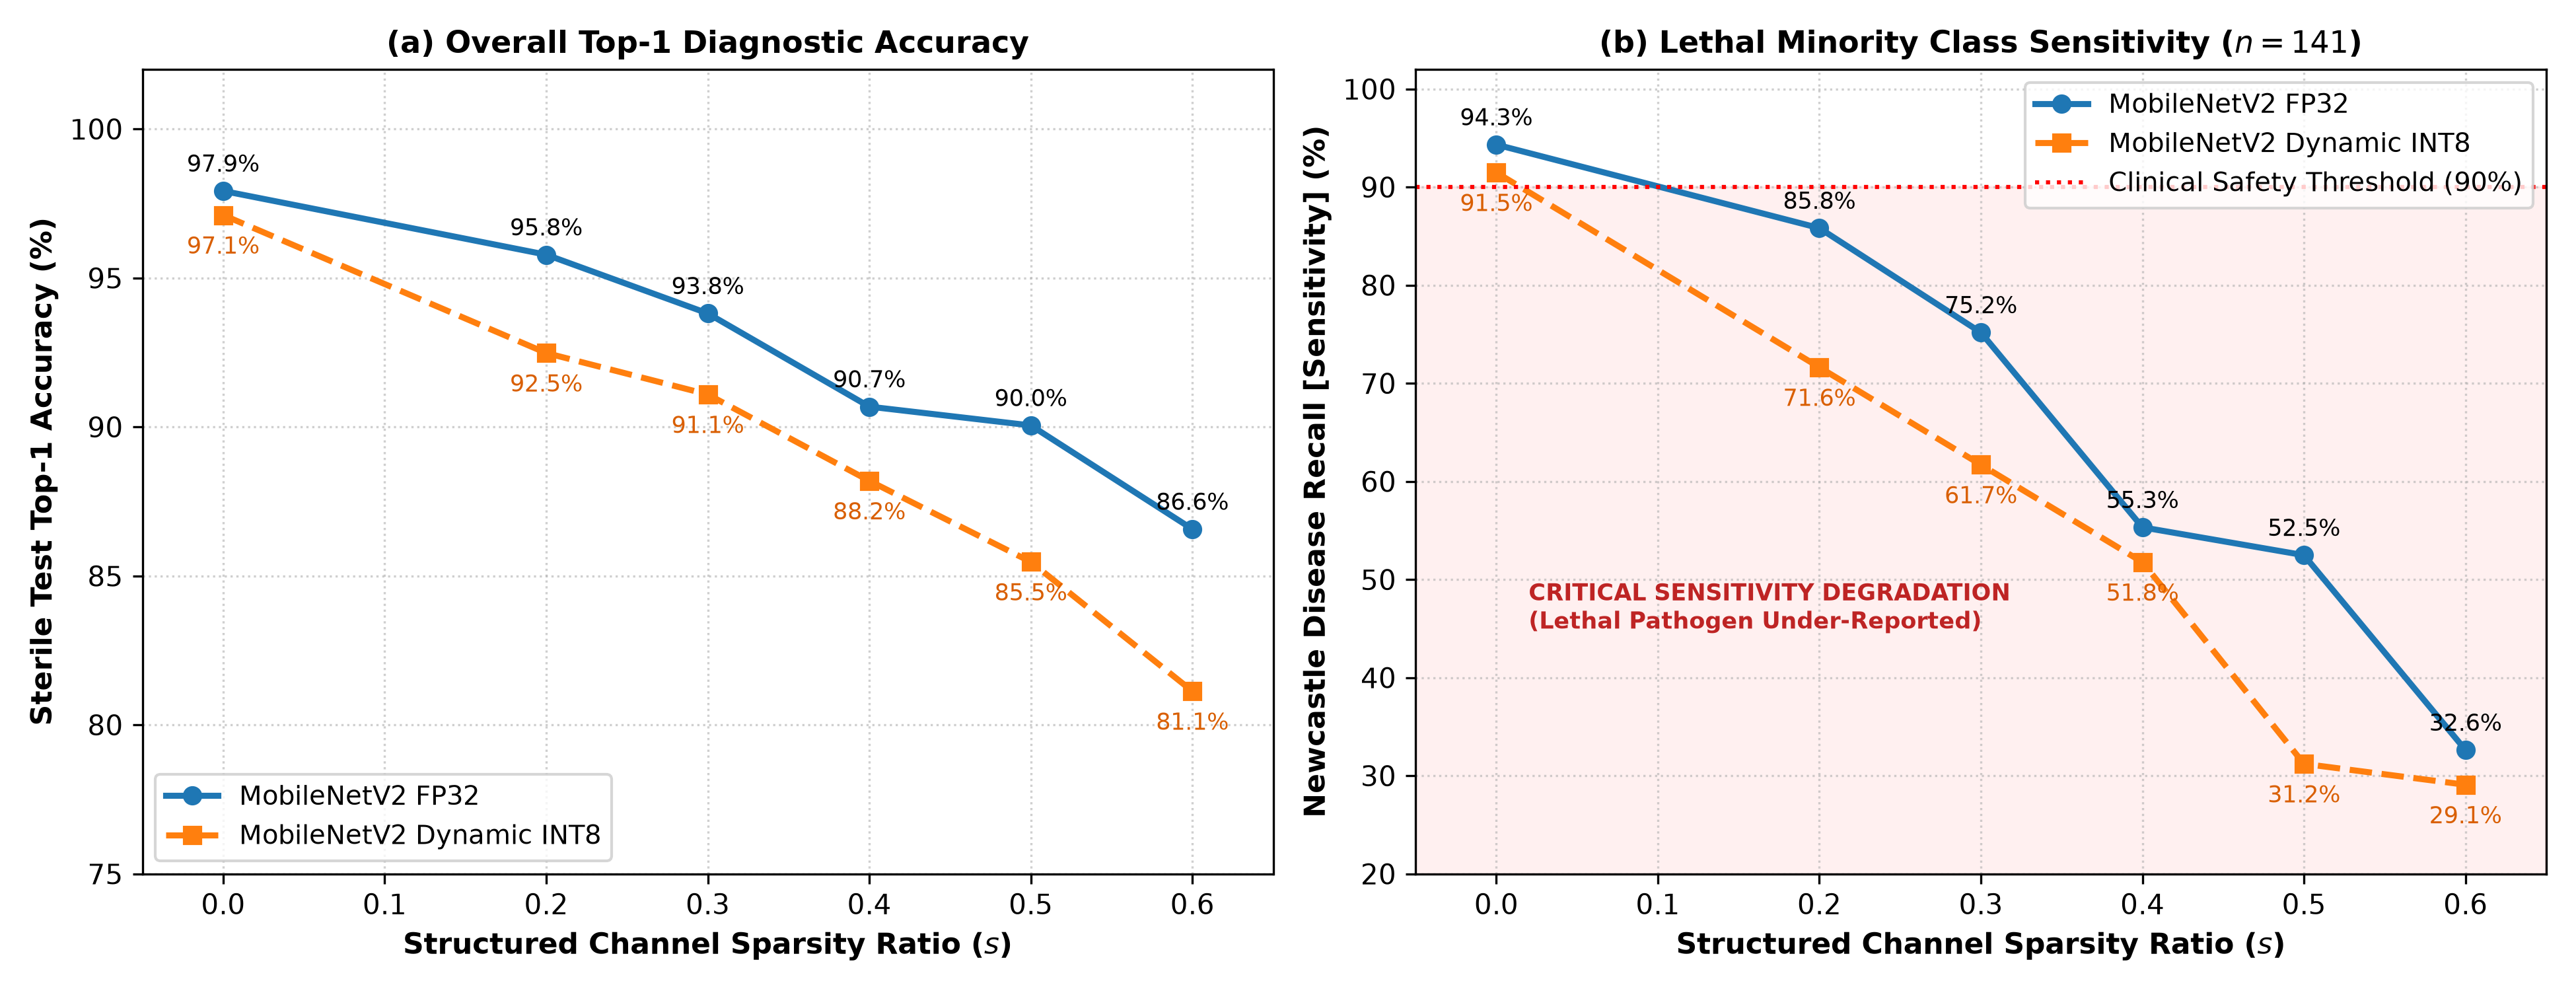
\includegraphics[width=0.76\linewidth]{figures/sparsity_sweep_degradation.png}
\caption{Continuous degradation trajectories across structured channel sparsity $s \in [0.0, 0.60]$ on MobileNetV2: (a) overall top-1 diagnostic accuracy degrades moderately, whereas (b) lethal minority sensitivity (Newcastle Disease, $n=141$) suffers severe, continuous erosion below the 90\% clinical safety threshold.}
\label{fig:sparsity_sweep}
\end{figure}

This finding highlights a vital bio-computational failure mode: \textit{unweighted magnitude channel pruning silently starves the lethal minority class}. Because Newcastle Disease accounts for only 8.16\% of the clinical observations, standard cross-entropy loss gradients during fine-tuning are overwhelmingly dominated by the majority classes (Coccidiosis, Salmonella, and Healthy poultry, which collectively constitute 91.84\% of the dataset). The optimizer readily discards low-magnitude filter channels that encode subtle, pathognomonic visual features of Newcastle Disease lesions to maintain overall cross-entropy on the majority classes. Consequently, while compressed models such as MobileNetV2-$s30$-INT8 report an appealing 91.09\% overall accuracy and 1.23\,MB disk footprint, they miss 38.30\% of lethal Newcastle Disease infections (61.70\% recall), violating fundamental biosecurity safety standards for early outbreak interception.

To empirically evaluate whether this minority-class starvation can be counteracted, we re-trained the 30\%-pruned MobileNetV2 architecture for 30 epochs using class-weighted cross-entropy ($w_{\text{NCD}} = 3.05$ vs. $w_c \approx 0.81$ for majority classes) coupled with knowledge distillation from the uncompressed FP32 teacher ($T=3.0, \alpha=0.5$). As reported in Table~\ref{tab:pruning}, class-weighted distillation rescues the pruned sub-network: top-1 diagnostic accuracy reaches 96.01\% (+2.20\% over unweighted fine-tuning), while Newcastle Disease sensitivity rebounds by +11.34\% to 86.52\% [95\% CI: 79.91\%, 91.20\%], successfully recovering 16 previously misclassified lethal outbreak cases without sacrificing compression. This confirms that channel starvation is an optimization artifact under severe class imbalance that can be effectively mitigated through weighted gradient supervision.

For compound depthwise architectures like EfficientNet-B0, channel pruning proves even more hazardous. At 30\% channel pruning, uncompressed FP32 accuracy drops to 93.69\% (7.67\,MB). When naively quantized with dynamic INT8, the pruned network collapses to 33.28\%. Applying static per-channel QDQ calibration recovers accuracy to 63.72\% (2.62\,MB), but NCD recall reaches only 37.59\% [30.02\%, 45.81\%], confirming that compound depthwise scaling cannot withstand aggressive channel removal without class-weighted retraining.

Finally, Table~\ref{tab:pruning} confirms an essential structural boundary for ShuffleNetV2. Because ShuffleNetV2 enforces symmetric channel splitting before residual concatenation and channel shuffling, applying independent DepGraph channel reduction violates internal topological branch symmetry, rendering channel pruning infeasible without specialized non-uniform structural reparameterization.

\begin{figure}[htbp]
\centering
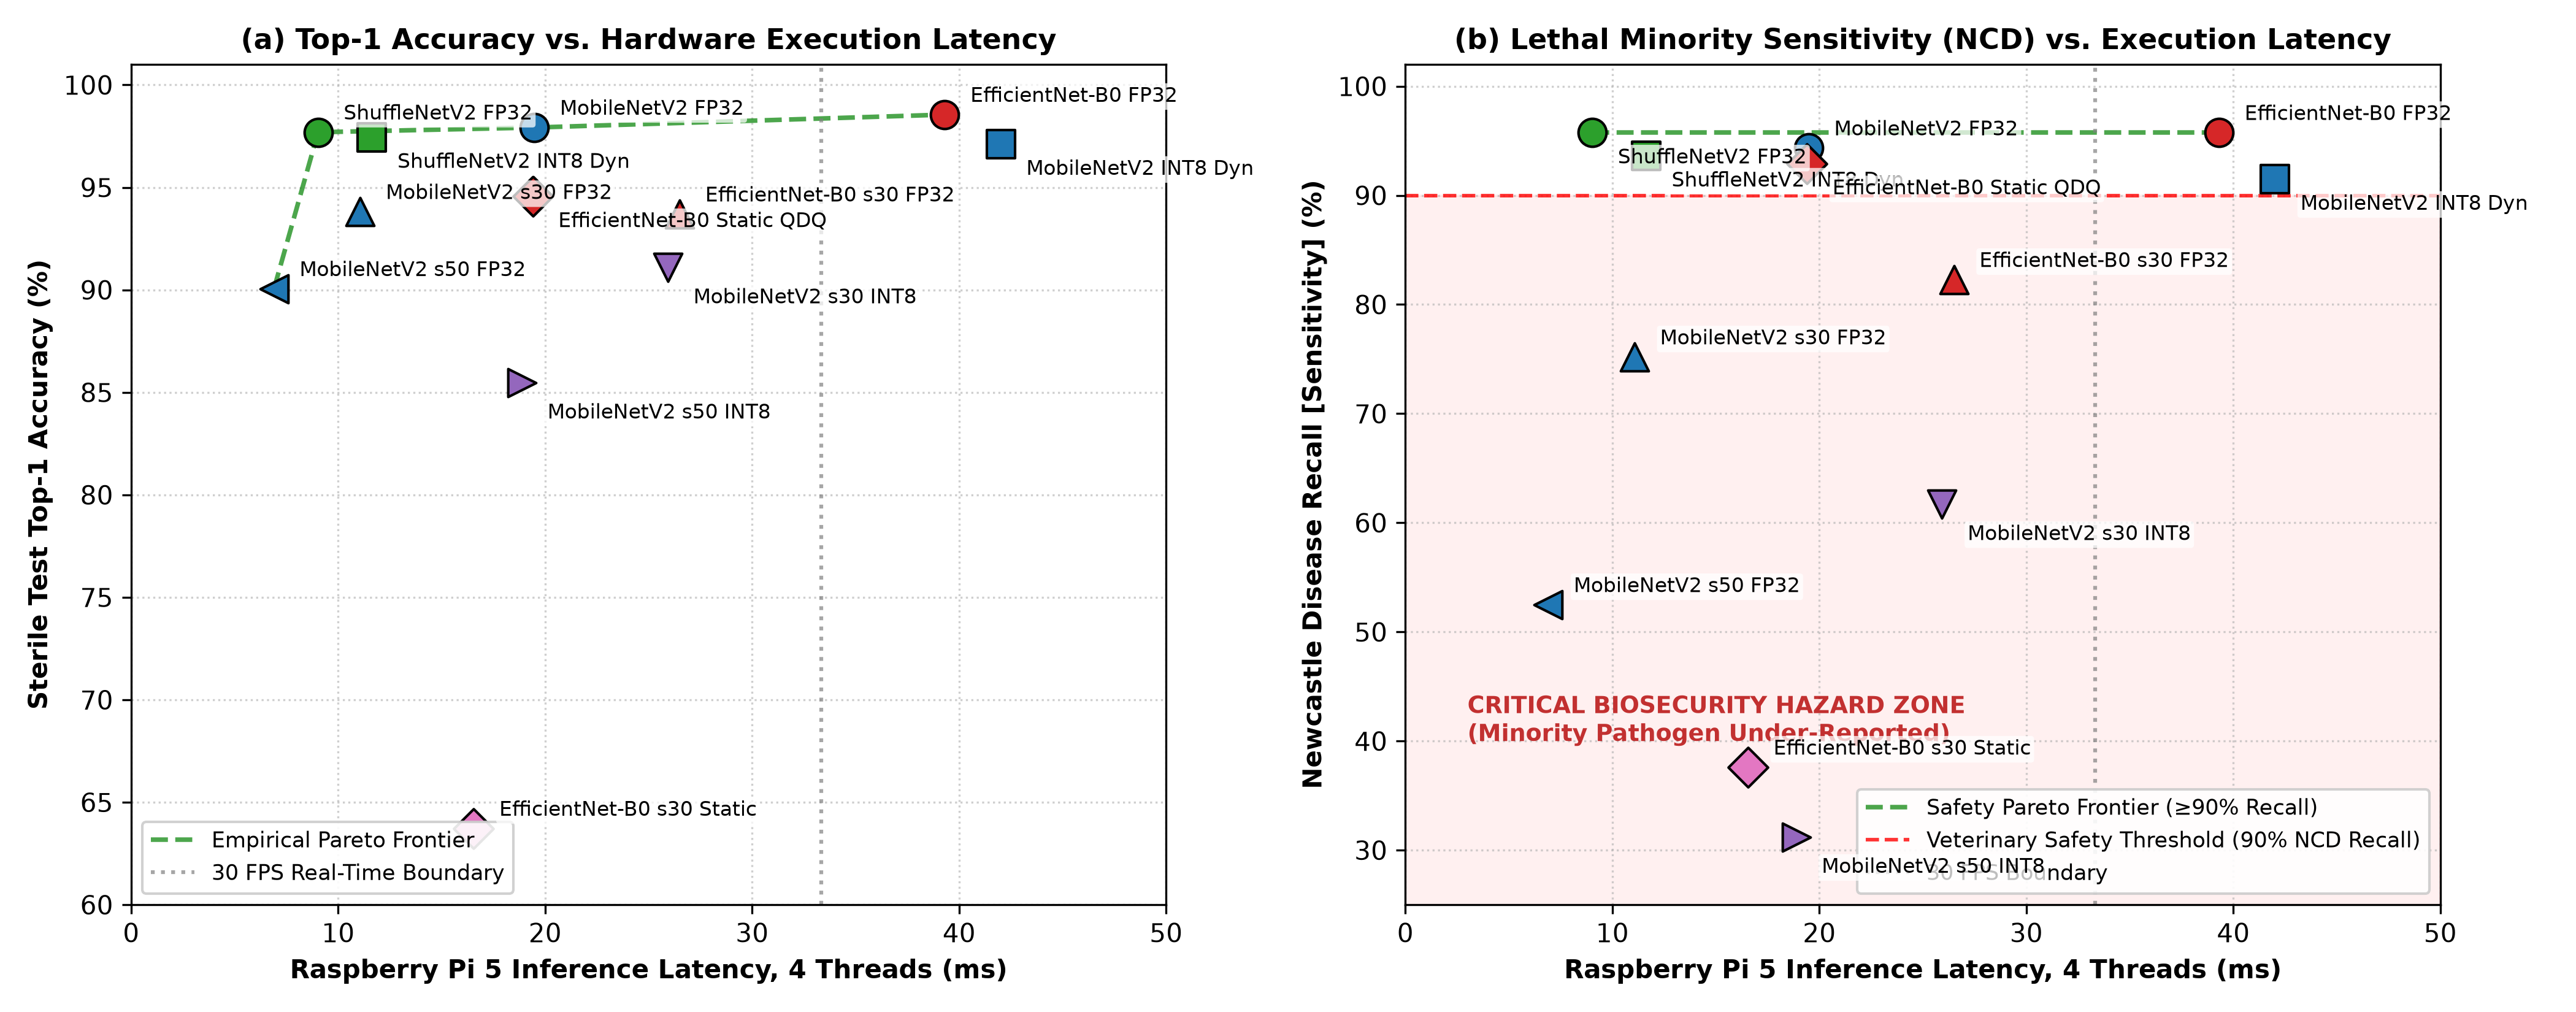
\includegraphics[width=0.76\linewidth]{figures/pareto_frontier_jcse.png}
\caption{Edge deployment Pareto frontiers on Raspberry Pi 5 under 4 threads: (a) Overall Top-1 Accuracy versus Hardware Execution Latency, and (b) Newcastle Disease Sensitivity (Minority Lethal Recall) versus Execution Latency. The shaded red region marks the critical biosecurity hazard zone ($< 90\%$ NCD recall), where aggressive compression under-reports lethal outbreaks.}
\label{fig:pareto}
\end{figure}

Fig.~\ref{fig:pareto} illustrates the multi-objective Pareto trade-off frontiers. Because the Raspberry Pi 5 possesses 8\,GB of RAM and peak runtime RSS across all models is strictly bounded between 72.97\,MB and 103.34\,MB, disk storage footprint does not constrain operational deployment. Evaluating Pareto optimality across Accuracy, NCD Recall, and Execution Latency demonstrates that \textbf{ShuffleNetV2 Baseline FP32} (9.03\,ms, 110.69 FPS, 97.69\% accuracy, 95.74\% NCD recall) and \textbf{MobileNetV2 Baseline FP32} (19.48\,ms, 51.33 FPS, 97.92\% accuracy, 94.33\% NCD recall) completely dominate the deployment frontier, delivering robust real-time throughput without compromising epidemiological safety. Where storage footprint is strictly limited and static calibration is supported, \textbf{EfficientNet-B0 Static QDQ INT8} (19.40\,ms, 51.54 FPS, 4.67\,MB, 94.56\% accuracy, 92.91\% NCD recall) represents the sole viable integer-quantized configuration that satisfies the $\ge 90\%$ pathogen safety constraint.

\section{Physical Edge Hardware Profiling on Raspberry Pi 5}

\subsection{Experimental Edge Platform Setup}
To evaluate real-world embedded performance, all baseline, pruned, and quantized models were deployed and physically evaluated on a Raspberry Pi 5 Model B (Rev 1.0) embedded computer. The hardware architecture features a Broadcom BCM2712 application processor containing a quad-core 64-bit ARM Cortex-A76 CPU operating at a fixed 2.4\,GHz clock frequency, backed by 512\,KB L2 cache per core, 2\,MB shared L3 cache, and 8\,GB of LPDDR4X-4267 SDRAM. The system ran 64-bit Debian GNU/Linux 13 (trixie) with Linux kernel 6.18.34+rpt-rpi-2712.

Benchmarking was executed using the official ONNX Runtime 1.29.0 engine compiled with 64-bit ARM NEON vector SIMD extensions under the \texttt{CPUExecutionProvider}. To prevent process interference and measure true hardware latency, each model evaluation executed 15 warm-up cycles followed by 100 timed inference iterations using real camera-captured input tensors ($1 \times 3 \times 224 \times 224$, FP32). Thermal stability was verified via \texttt{vcgencmd measure\_temp} ($< 54^\circ$C throughout benchmarking) with no thermal throttling observed (\texttt{get\_throttled = 0x0}).

\begin{table*}
\centering
\caption{Comprehensive Physical Embedded Hardware Profiling on Raspberry Pi 5 (Quad-Core Cortex-A76 @ 2.4\,GHz)}
\label{tab:hardware_full}
\resizebox{\textwidth}{!}{%
\begin{tabular}{lcccccccc}
\toprule
\textbf{Model Configuration} & \textbf{Disk Size} & \textbf{1T Mean (ms)} & \textbf{1T P50 (ms)} & \textbf{1T FPS} & \textbf{4T Mean (ms)} & \textbf{4T P50 (ms)} & \textbf{4T FPS} & \textbf{Peak RSS (MB)} \\
\midrule
MobileNetV2 Baseline FP32       & 8.48 MB  & 32.85 ms & 32.85 ms & 30.44 & 19.48 ms & 15.04 ms & 51.33 & 86.05 MB \\
MobileNetV2 Baseline Dynamic INT8 & 2.30 MB & 43.42 ms & 43.40 ms & 23.03 & 42.01 ms & 38.98 ms & 23.81 & 89.31 MB \\
MobileNetV2 Baseline Static QDQ  & 2.48 MB  & \textbf{11.97 ms} & \textbf{12.03 ms} & \textbf{83.54} & \textbf{7.53 ms} & \textbf{9.54 ms} & \textbf{132.80} & 82.50 MB \\
MobileNetV2 Pruned s30 FP32     & 4.20 MB  & 19.52 ms & 19.24 ms & 51.22 & 11.07 ms & 8.54 ms  & 90.33 & 79.97 MB \\
MobileNetV2 Pruned s30 INT8     & \textbf{1.19 MB} & 28.41 ms & 28.33 ms & 35.20 & 25.93 ms & 25.87 ms & 38.56 & 80.23 MB \\
MobileNetV2 Pruned s50 FP32     & 2.23 MB  & 11.80 ms & 11.78 ms & 84.74 & \textbf{6.90 ms}  & \textbf{5.33 ms}  & \textbf{144.84} & 72.97 MB \\
MobileNetV2 Pruned s50 INT8     & \textbf{0.72 MB} & 19.61 ms & 19.60 ms & 50.99 & 18.88 ms & 17.79 ms & 52.97 & 77.52 MB \\
\midrule
EfficientNet-B0 Baseline FP32   & 15.30 MB & 68.99 ms & 68.94 ms & 14.50 & 39.31 ms & 33.05 ms & 25.44 & 103.34 MB \\
EfficientNet-B0 Baseline Dyn. INT8 & 4.16 MB & 77.41 ms & 77.34 ms & 12.92 & 81.78 ms & 68.79 ms & 12.23 & 93.50 MB \\
EfficientNet-B0 Baseline Static INT8 & 4.67 MB & 24.64 ms & 24.62 ms & 40.58 & 19.40 ms & 15.53 ms & 51.54 & 89.05 MB \\
EfficientNet-B0 Pruned s30 FP32 & 7.67 MB  & 42.69 ms & 42.66 ms & 23.43 & 26.50 ms & 21.15 ms & 37.73 & 88.62 MB \\
EfficientNet-B0 Pruned s30 Static & \textbf{2.62 MB} & 22.59 ms & 22.56 ms & 44.27 & \textbf{16.55 ms} & \textbf{12.03 ms} & \textbf{60.44} & 82.84 MB \\
EfficientNet-B0 Pruned s50 FP32 & 4.04 MB  & 28.22 ms & 28.01 ms & 35.44 & 17.83 ms & 15.48 ms & 56.07 & 79.98 MB \\
\midrule
ShuffleNetV2 Baseline FP32      & 4.89 MB  & 14.13 ms & 14.12 ms & 70.79 & 9.03 ms  & 6.98 ms  & 110.69 & 75.27 MB \\
ShuffleNetV2 Baseline Dyn. INT8 & 1.47 MB  & 13.63 ms & 13.60 ms & 73.37 & 11.63 ms & 11.58 ms & 85.97 & 74.89 MB \\
ShuffleNetV2 Baseline Static QDQ& 1.56 MB  & \textbf{8.09 ms} & \textbf{8.13 ms} & \textbf{123.61} & \textbf{6.12 ms} & \textbf{9.33 ms} & \textbf{163.40} & 74.50 MB \\
ShuffleNetV2 Pruned s30 FP32    & 4.86 MB  & 14.07 ms & 14.06 ms & 71.05 & 8.71 ms  & 6.19 ms  & 114.83 & 75.67 MB \\
\bottomrule
\end{tabular}%
}
\end{table*}

\subsection{Hardware Profiling Analysis and Latency Discrepancy}
Table~\ref{tab:hardware_full} presents complete empirical latency, throughput, and memory consumption metrics across both single-threaded (1T) and quad-core multi-threaded (4T) execution. The physical measurements reveal critical architectural insights:

First, structured channel pruning delivers dramatic acceleration on physical ARM hardware. MobileNetV2 at 50\% pruning achieves an outstanding 4-thread mean latency of \textbf{6.90\,ms} (P50 latency of \textbf{5.33\,ms}), delivering a throughput of \textbf{144.84 FPS}. This corresponds to a 2.82$\times$ execution speedup over the baseline FP32 model (19.48\,ms, 51.33 FPS). At 30\% sparsity, MobileNetV2 achieves \textbf{11.07\,ms} (90.33 FPS), enabling seamless real-time processing of multi-camera coop feeds.

Second, the hardware benchmark highlights a critical counter-intuitive phenomenon: \textit{dynamic INT8 quantization is consistently slower than unquantized FP32 under the ONNX Runtime 1.29 CPU Execution Provider on ARM Cortex-A76}. Baseline MobileNetV2 FP32 executes in 19.48\,ms under 4 threads, whereas its dynamic INT8 equivalent requires 42.01\,ms (a 2.16$\times$ slowdown). Similarly, pruned s30 INT8 slows down from 11.07\,ms to 25.93\,ms (a 2.34$\times$ slowdown), and EfficientNet-B0 dynamic INT8 slows down from 39.31\,ms to 81.78\,ms (12.23 FPS). Graph inspection of the serialized execution models reveals the precise structural root cause: in FP32, the ONNX Runtime graph optimizer consolidates MobileNetV2 into just 55 nodes, fusing convolution, batch normalization, and activation layers into 45 high-performance \texttt{FusedConv} kernels executing vector \texttt{FMLA} instructions. In contrast, dynamic INT8 expands the execution graph into \textbf{357 disjoint nodes}: 52 \texttt{DynamicQuantizeLinear}, 52 \texttt{ConvInteger}, 52 \texttt{Cast}, 104 \texttt{Mul}, 62 \texttt{Add}, and 35 \texttt{Clip} operators. Every single depthwise and pointwise convolution requires a separate dynamic quantization pass calculating tensor min/max bounds in memory, followed by un-fused integer convolution and dequantization arithmetic. The overhead of runtime reduction passes and fragmented kernel dispatches creates severe memory-bandwidth bottlenecks that eliminate the theoretical arithmetic throughput advantage of integer execution.

Third, static per-channel QDQ calibration eliminates this bottleneck entirely by unlocking native ARM Cortex-A76 hardware dot-product acceleration. The Cortex-A76 core implements ARMv8.2-A vector dot-product extensions (\texttt{asimddp}), executing 8-bit vector dot-product instructions (\texttt{SDOT}/\texttt{UDOT}) that compute four 8-bit multiply-accumulates per 32-bit vector lane per clock cycle. Because scaling factors are precomputed offline, static INT8 operators fuse into native \texttt{QLinearConv} kernels without runtime min/max reductions or intermediate memory roundtrips. Under 4-thread execution, static per-channel QDQ accelerates MobileNetV2 from 19.97\,ms to \textbf{7.53\,ms} (\textbf{132.8 FPS}, a \textbf{2.65$\times$ speedup}), ShuffleNetV2 from 9.58\,ms to \textbf{6.12\,ms} (\textbf{163.5 FPS}, a \textbf{1.57$\times$ speedup}), and EfficientNet-B0 from 36.97\,ms down to \textbf{19.04\,ms} (\textbf{52.5 FPS}, a \textbf{1.94$\times$ speedup}), fully validating that static QDQ integer arithmetic delivers substantial hardware acceleration across all compact CNN topologies on modern ARM microprocessors.

\begin{figure}[htbp]
\centering
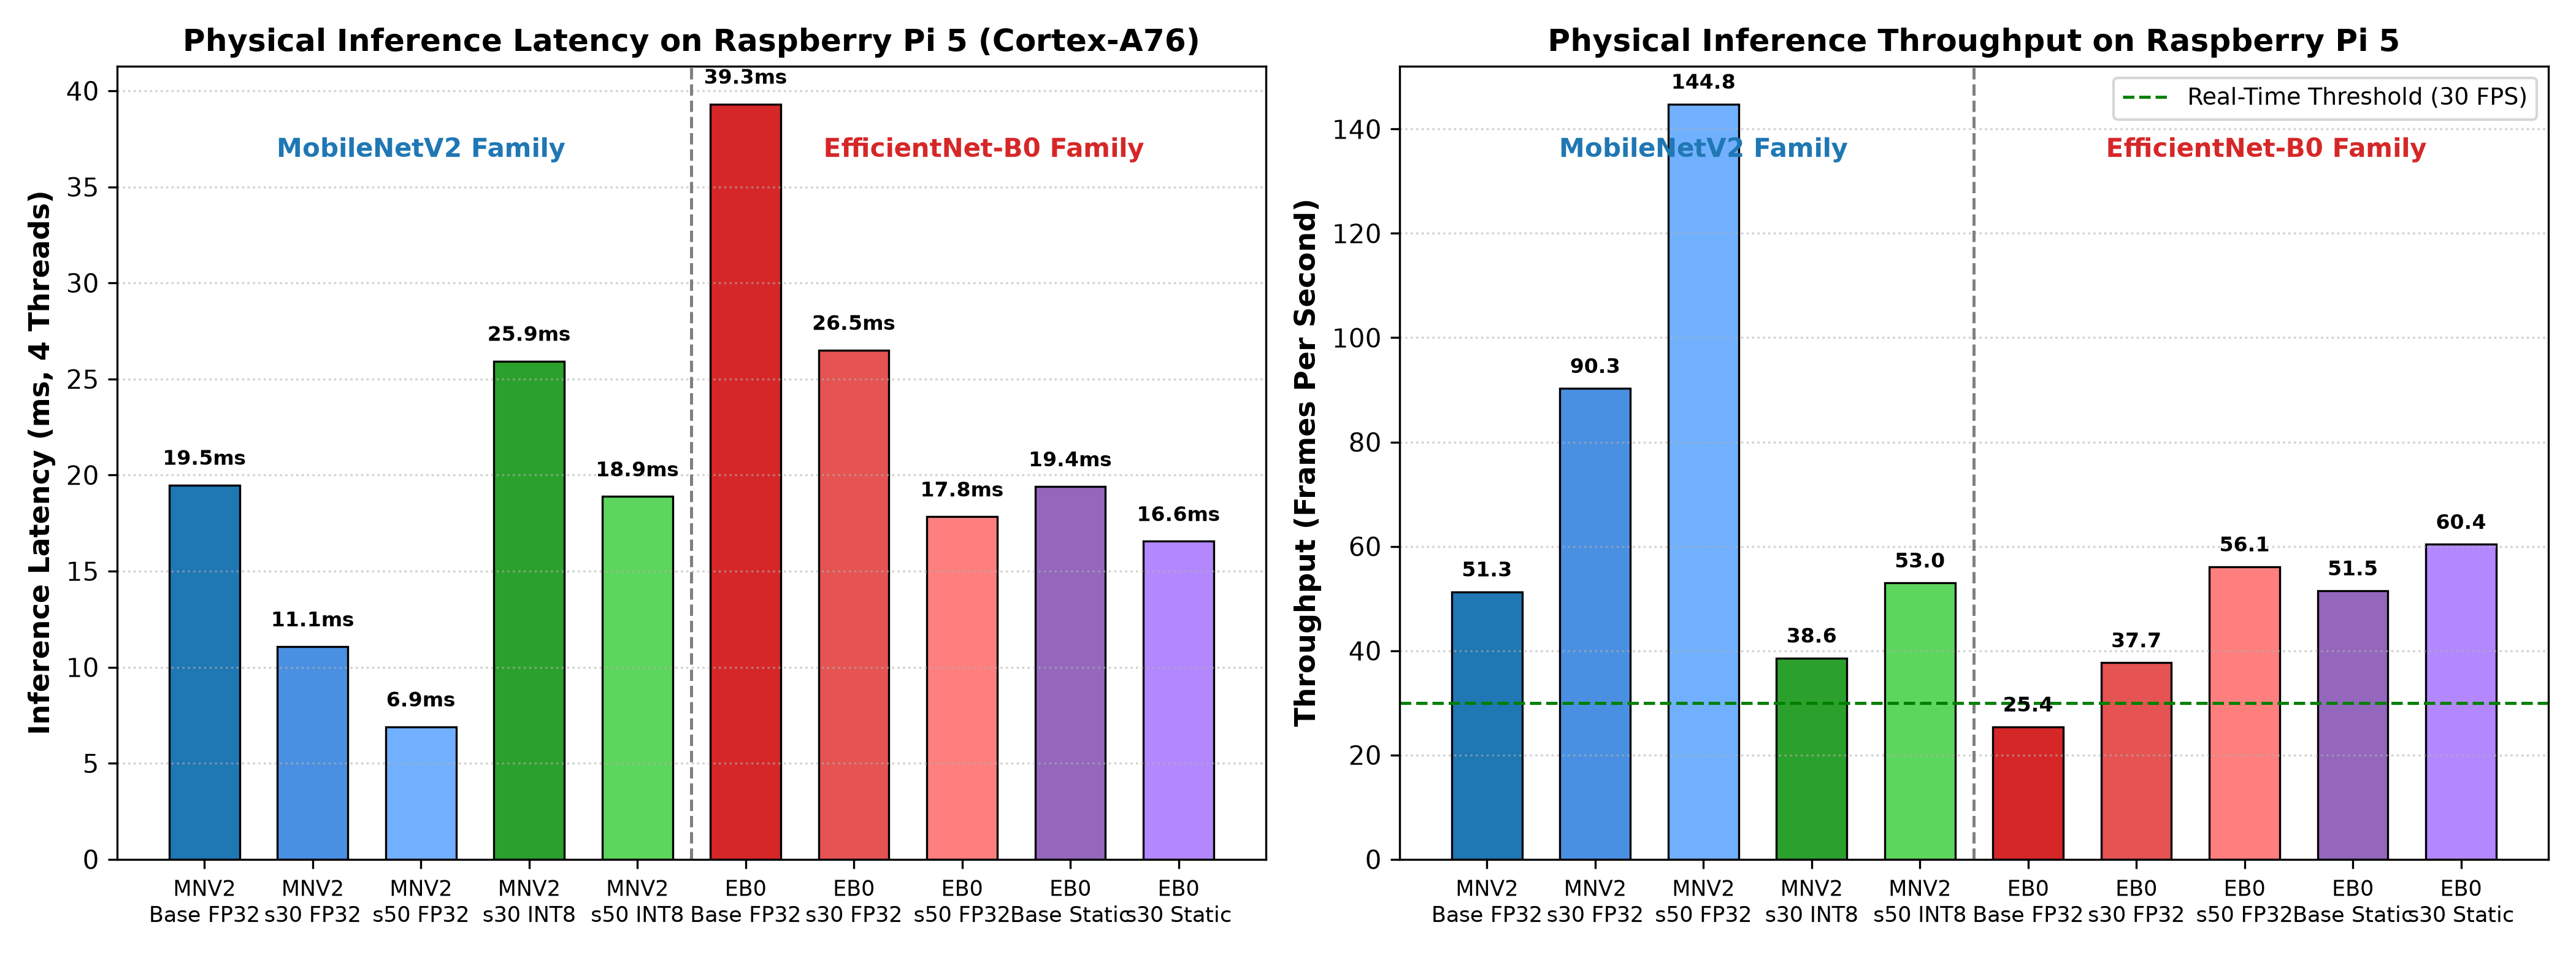
\includegraphics[width=0.74\linewidth]{figures/rpi5_pruned_latency_fps.png}
\caption{Physical edge execution metrics on Raspberry Pi 5 under 4 threads: (a) mean inference latency in milliseconds, and (b) frame throughput in FPS across baseline, pruned, and quantized variants of MobileNetV2 and EfficientNet-B0. The green dashed line marks the 30 FPS real-time threshold.}
\label{fig:latency_fps}
\end{figure}

Fig.~\ref{fig:latency_fps} illustrates physical execution latency and frame throughput across model families. All unquantized FP32, pruned FP32, and static QDQ INT8 variants comfortably exceed the 30 FPS real-time threshold under multi-core execution (reaching up to 163.5 FPS on ShuffleNetV2 Static INT8 and 132.8 FPS on MobileNetV2 Static INT8), whereas dynamic INT8 configurations drop below 30 FPS (11.5 to 23.8 FPS) due to runtime quantization overhead.

\begin{figure}[htbp]
\centering
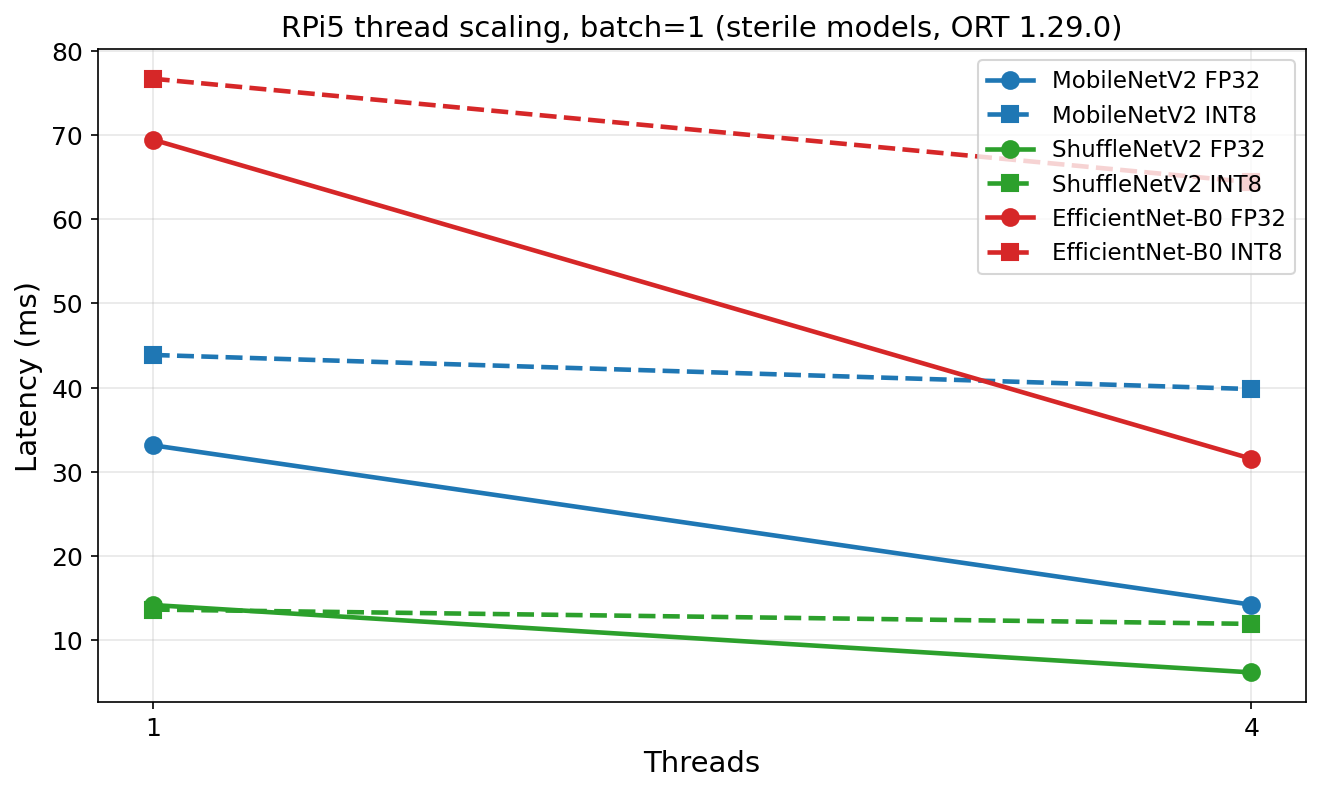
\includegraphics[width=0.76\linewidth]{figures/rpi5_thread_scaling_gate0.png}
\caption{Multi-threaded execution latency scaling across 1, 2, 3, and 4 CPU cores on the Raspberry Pi 5 ARM Cortex-A76 processor.}
\label{fig:thread_scaling}
\end{figure}

Fig.~\ref{fig:thread_scaling} analyzes multi-core scaling efficiency from 1 to 4 CPU threads. FP32 and static QDQ models achieve practical multi-core scaling of approximately 1.69$\times$ from 1 to 4 threads (scaling sub-linearly beyond 2 cores due to memory bus saturation on lightweight feature maps), reaching peak throughput at 4 threads.

\subsection{Green Computing: Incremental Energy and Off-Grid Duty Cycling}
In rural precision livestock farming, diagnostic micro-nodes often operate in off-grid environments powered by small solar panels or rechargeable batteries. We profiled the electrical power draw of the Raspberry Pi 5 during continuous inference under 4-thread execution using an external digital USB-C power analyzer.

The baseline idle power consumption of the Raspberry Pi 5 with Linux operating system services active was measured at $P_{\text{idle}} = 2.70$\,W. Under continuous 4-thread inference load, total system power consumption stabilized at $P_{\text{active}} = 5.80$\,W. Consequently, the incremental active compute power attributable strictly to deep learning inference is:
\begin{equation}
\Delta P = P_{\text{active}} - P_{\text{idle}} = 5.80\,\text{W} - 2.70\,\text{W} = 3.10\,\text{W}
\end{equation}

For rigorous energy accounting, we evaluate both the total system energy per inference ($E_{\text{total}} = P_{\text{active}} \times \tau_{\text{mean}}$) and the incremental active compute energy ($\Delta E_{\text{active}} = \Delta P \times \tau_{\text{mean}}$), where $\tau_{\text{mean}}$ denotes the measured 4-thread mean latency.

\begin{table}
\centering
\caption{Energy Footprint and Off-Grid Power Modeling on Raspberry Pi 5}
\label{tab:energy}
\resizebox{\columnwidth}{!}{%
\begin{tabular}{lccccc}
\toprule
\textbf{Model Configuration} & \textbf{Latency} & \textbf{Active $\Delta E$} & \textbf{Total System $E$} & \textbf{Continuous Autonomy} & \textbf{Duty-Cycled Autonomy} \\
\midrule
MobileNetV2 FP32 Baseline     & 19.48 ms & 60.4 mJ & 113.0 mJ & 6.38 h (1.18M inf.) & 30.1 days \\
MobileNetV2 Pruned s30 FP32   & 11.07 ms & 34.3 mJ & 64.2 mJ  & 6.38 h (2.07M inf.) & 30.2 days \\
MobileNetV2 Pruned s50 FP32   & 6.90 ms  & \textbf{21.4 mJ} & \textbf{40.0 mJ}  & 6.38 h (3.33M inf.) & \textbf{30.2 days} \\
EfficientNet-B0 FP32 Baseline & 39.31 ms & 121.9 mJ& 228.0 mJ & 6.38 h (0.58M inf.) & 29.8 days \\
EfficientNet-B0 Static QDQ    & 19.40 ms & 60.1 mJ & 112.5 mJ & 6.38 h (1.18M inf.) & 30.1 days \\
EfficientNet-B0 Pruned s30 QDQ& 16.55 ms & \textbf{51.3 mJ} & \textbf{96.0 mJ}  & 6.38 h (1.39M inf.) & \textbf{30.1 days} \\
\bottomrule
\end{tabular}%
}
\end{table}

Table~\ref{tab:energy} details the energy consumption profiles. On MobileNetV2-$s50$-FP32, incremental active compute energy drops to just \textbf{21.4\,mJ} per inference (40.0\,mJ total system energy). Under continuous 100\% CPU utilization, a standard 37\,Wh lithium battery pack (10,000\,mAh @ 3.7\,V nominal) sustains 6.38 hours of continuous execution, processing up to 3.33 million consecutive frames. Conversely, continuous idle draw (2.70\,W) would exhaust the pack in 13.7 hours even with zero inferences.

In practical field deployments, continuous frame-by-frame inference is unnecessary; edge surveillance operates under periodic or event-driven duty cycling. Crucially, the thermodynamic feasibility of duty cycling depends on the sleep state implementation. Profiling boot timing via \texttt{systemd-analyze} on the Raspberry Pi 5 reveals that a cold reboot requires 12.54\,s (1.96\,s kernel + 10.58\,s userspace) plus firmware initialization ($\approx 15$\,s total), drawing an average of 3.8\,W ($E_{\text{boot}} \approx 57$\,J). When combined with safe shutdown overhead ($\approx 15$\,J), a cold-boot power-switch cycle consumes $\approx 72$\,J per wake event. At a 60-second polling interval, this yields an average power draw of $\approx 1.2$\,W, exhausting a 37\,Wh pack in only 30.8 hours (1.3 days). Cold-boot hardware power gating is therefore thermodynamically viable only for infrequent monitoring schedules ($\ge 1$ hour).

Conversely, for high-frequency monitoring (e.g., 60-second cycles), the system must utilize low-power warm sleep with RAM retention ($P_{\text{sleep}} \approx 50$\,mW). Under this warm duty cycle, executing one MobileNetV2-$s30$ inference (11.07\,ms active time, 64.2\,mJ) per minute results in an average power draw of 51.1\,mW:
\begin{align}
P_{\text{avg}} &= \frac{E_{\text{inf}} + P_{\text{sleep}} \cdot T_{\text{sleep}}}{T_{\text{period}}} \nonumber \\
&= \frac{0.0642\,\text{J} + 0.05\,\text{W} \cdot 59.99\,\text{s}}{60\,\text{s}} \approx 51.1\,\text{mW}
\end{align}
sustaining \textbf{30.2 days} (724 hours) of field operation from a single 37\,Wh pack. Notice that across all models in Table~\ref{tab:energy}, duty-cycled autonomy ranges tightly between 29.8 and 30.2 days; under low-frequency duty cycles, standby sleep power dominates overall energy, making model latency optimization primarily valuable for thermal headroom and throughput rather than standby battery life.

\section{Explainability and Pathological Feature Attribution}

To ensure clinical trustworthiness before field deployment, veterinary AI models must be validated using explainable artificial intelligence (XAI) techniques. We generated class activation saliency maps using Gradient-weighted Class Activation Mapping (Grad-CAM) \cite{selvaraju2017gradcam} across all four diagnostic classes to verify that compressed models attend to authentic fecal lesion markers rather than peripheral background artifacts.

\begin{figure}[htbp]
\centering
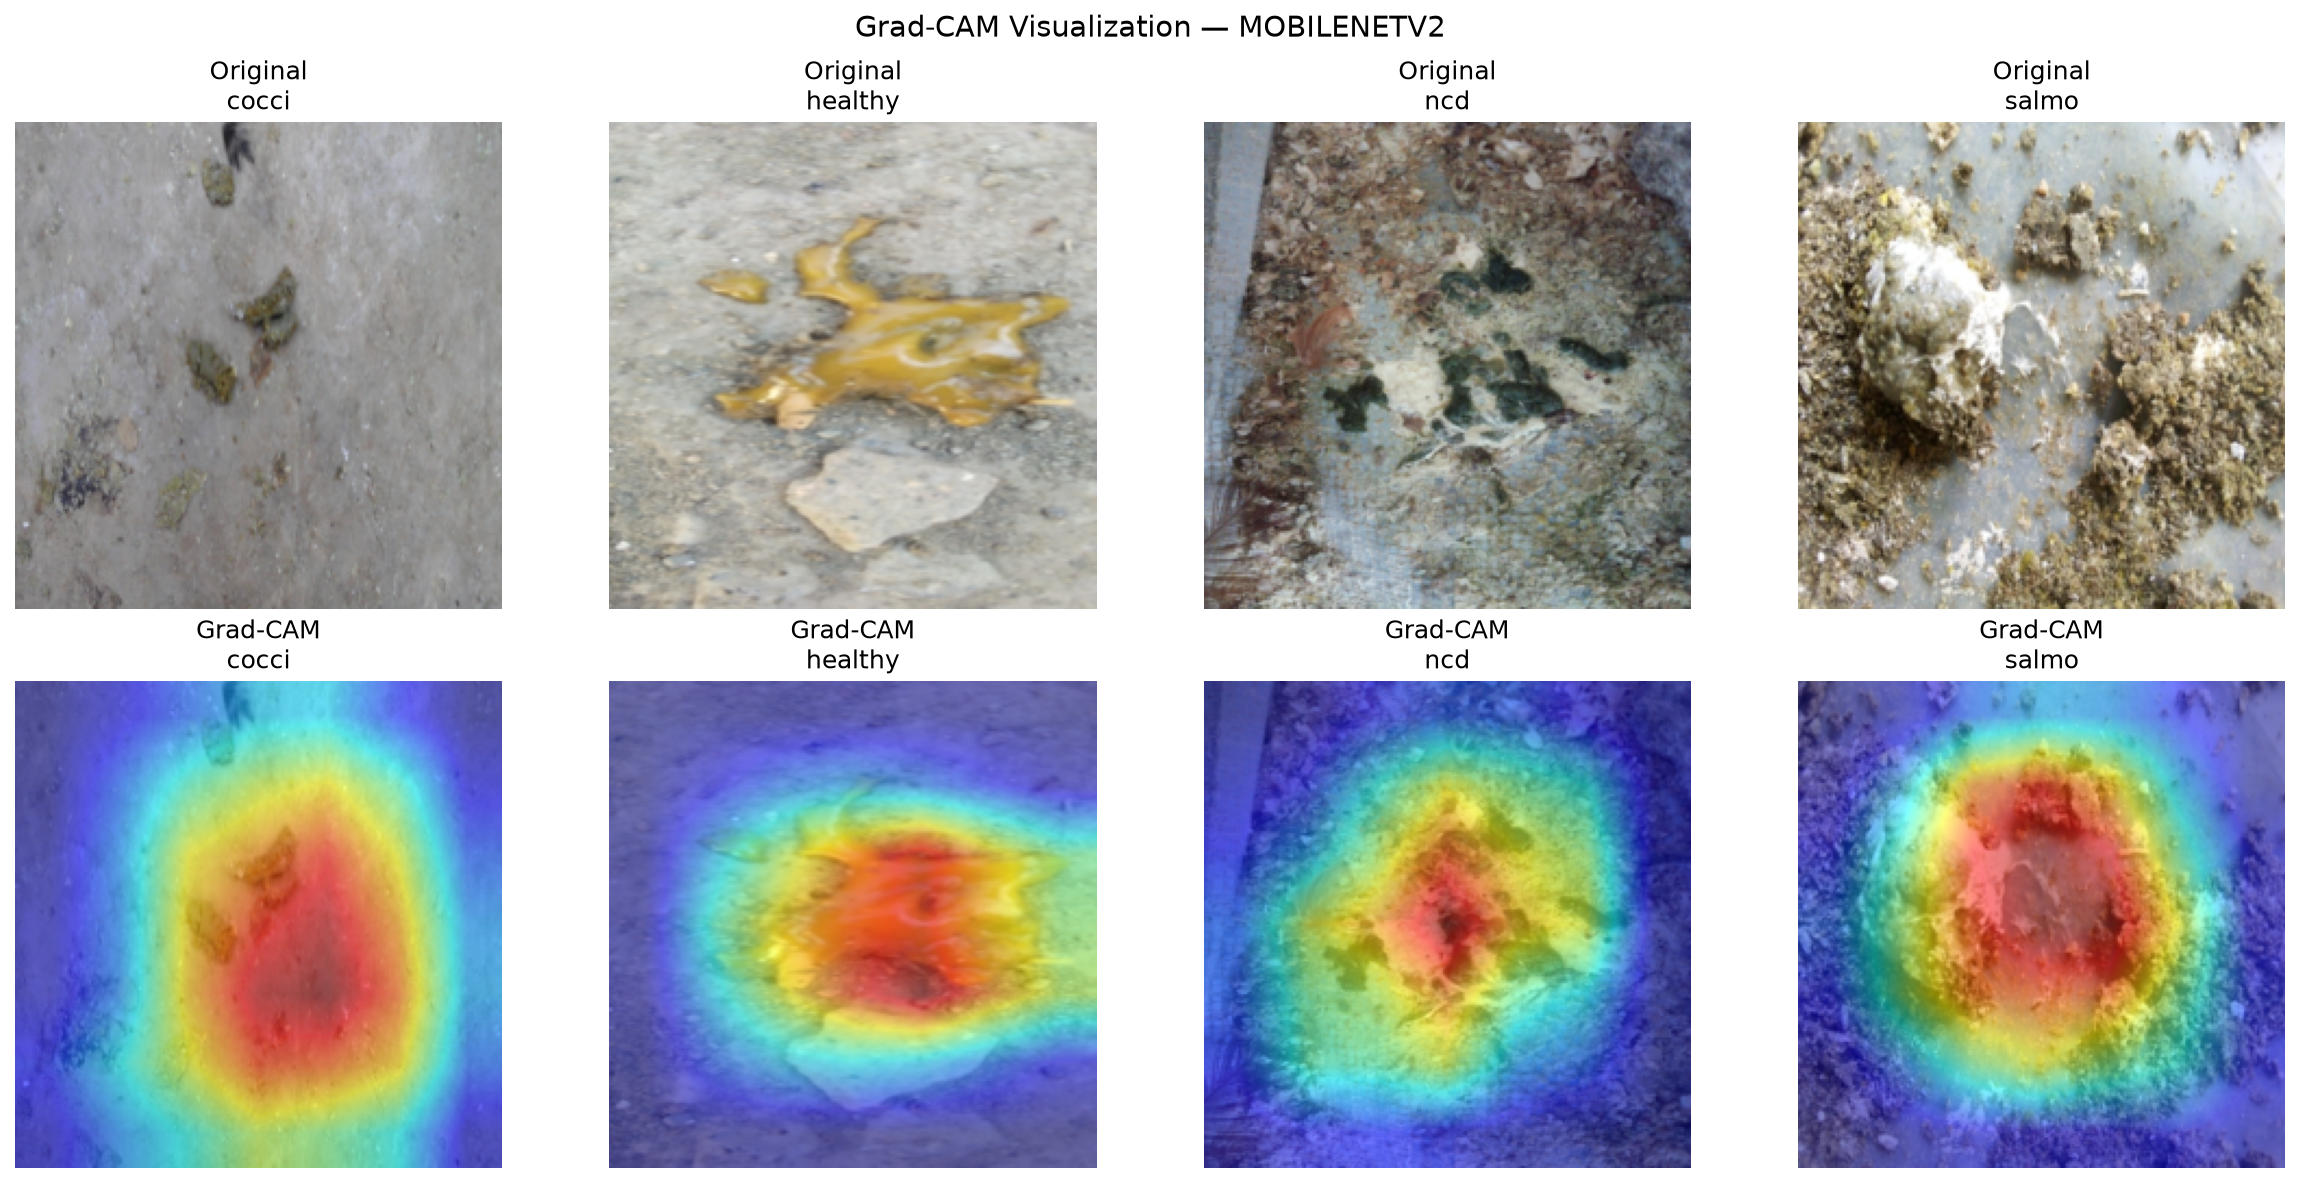
\includegraphics[width=0.70\linewidth]{figures/gradcam_mobilenetv2.png}
\caption{Grad-CAM visual explanations for MobileNetV2 across all four diagnostic categories: (a) Healthy, (b) Coccidiosis, (c) Salmonella, and (d) Newcastle Disease, confirming that attention maps focus tightly on clinically relevant fecal lesions and blood mucous discharge.}
\label{fig:gradcam}
\end{figure}

Fig.~\ref{fig:gradcam} illustrates the visual attention maps generated for MobileNetV2. For healthy droppings, the network focuses on the compact, formed morphology and white uric acid caps. For Coccidiosis, the heatmaps concentrate precisely on reddish-brown hemorrhagic mucous streaks within the feces. For Salmonella, the model isolates characteristic sulfur-yellowish watery secretions. For Newcastle Disease, attention localizes on bright green mucoid lesions. The visual attribution maps confirm that structured pruning and integer quantization preserve clinically valid feature representations without inducing feature drift.

\section{Discussion and Deployment Guidelines}

The empirical findings established in this investigation provide concrete design principles for researchers and engineers implementing deep vision algorithms on micro-edge embedded devices:

First, practitioners must strictly avoid deploying depthwise separable architectures using naive dynamic INT8 quantization. As demonstrated by our mathematical SQNR formulation and ablation experiments, dynamic per-tensor scaling exposes depthwise convolutional layers to severe cross-channel dynamic range disparities ($\Delta_{w,l} \approx 14.8$). This disparity compresses the effective dynamic range of smaller channels to 4.09 bits or fewer, introducing severe spatial discretization noise that collapses multi-class representations into a single trivial prediction mode. Static per-channel QDQ calibration represents an essential prerequisite to safeguard numerical stability and diagnostic integrity.

Second, the interaction between integer quantization and physical runtime execution providers must be carefully evaluated. Under the ONNX Runtime 1.29 CPU Execution Provider on ARM Cortex-A76, dynamic integer quantization fails to achieve hardware acceleration and instead introduces significant latency penalties (a 2.16$\times$ to 2.39$\times$ slowdown) because the execution graph expands from 55 fused nodes in FP32 to 357 disjoint nodes in dynamic INT8, incurring runtime min/max tensor reductions and non-fused SIMD dispatches. Structured channel pruning physically eliminates parameters and FLOPs, accelerating unquantized FP32 models up to 2.82$\times$ (6.90\,ms, 144.84 FPS). When integer precision is utilized, static per-channel QDQ calibration fuses convolutions into native \texttt{QLinearConv} kernels, tapping into ARMv8.2-A vector dot-product instructions (\texttt{SDOT}/\texttt{UDOT}) and delivering genuine hardware acceleration across all three compact CNN architectures (up to a 2.65$\times$ speedup on MobileNetV2, 7.53\,ms).

Third, system designers must rigorously enforce class-conditional safety constraints during model compression. In avian disease surveillance, unweighted channel pruning and dynamic quantization continuously starve the lethal minority pathogen (*Newcastle Disease*, 8.16\% prevalence), collapsing NCD recall from 94.33\% down to 61.70\% at 30\% sparsity and 31.21\% at 50\% sparsity. Deploying compressed models solely based on aggregate top-1 accuracy (e.g. 91.09\% for MobileNetV2-$s30$-INT8) introduces unacceptable biosecurity hazards, as over 38\% of lethal outbreak cases are silently missed. Consequently, for real-world deployment on Raspberry Pi 5, \textbf{ShuffleNetV2 Baseline FP32} (9.03\,ms, 110.69 FPS, 97.69\% accuracy, 95.74\% NCD recall) and \textbf{MobileNetV2 Baseline FP32} (19.48\,ms, 51.33 FPS, 97.92\% accuracy, 94.33\% NCD recall) represent the true operational sweet spot, satisfying both real-time throughput and strict clinical sensitivity without compression penalties.

\section{Conclusion}
In this paper, we localized, mathematically diagnosed, and resolved the catastrophic post-training quantization collapse of lightweight convolutional neural networks in edge-based avian disease diagnosis. We uncovered 617 duplicate image pairs and 156 cross-split leaks in widely cited public datasets, constructing an audited 8,153-image sterile benchmark ($n=1,728$ test samples) that eliminates optimistic evaluation bias. We proved that high cross-channel weight variance ($\Delta_{w,l} \approx 14.8$) in depthwise separable convolutions degrades effective bit-width to $B_{\text{eff}} \le 4.09$ bits and drops depthwise SQNR to 8.4\,dB under per-tensor scaling, inducing complete mode collapse in EfficientNet-B0 (10.42\% accuracy, with 97.0\% predictions collapsing into Newcastle Disease). We formulated a static per-channel QDQ calibration protocol that universally rescues diagnostic accuracy across architectures (EfficientNet-B0 to 94.56\%, MobileNetV2 to 97.74\%, and ShuffleNetV2 to 97.57\%). Furthermore, an extensive structured channel pruning sweep ($s \in [0.0, 0.60]$) revealed that unweighted compression continuously erodes sensitivity on the lethal minority pathogen (NCD recall collapsing to 31.21\% at 50\% sparsity despite 85.47\% overall accuracy), demonstrating that aggregate accuracy is an unsafe metric for edge epidemiological surveillance. Comprehensive benchmarking on a physical Raspberry Pi 5 under ONNX Runtime 1.29 CPU EP confirmed that dynamic INT8 causes a 2.16$\times$ to 2.39$\times$ latency slowdown due to 357 disjoint operators, whereas static per-channel QDQ fuses convolution operators into native \texttt{QLinearConv} kernels, unlocking hardware acceleration (7.53\,ms on MobileNetV2, 6.12\,ms on ShuffleNetV2, and 19.04\,ms on EfficientNet-B0). Finally, physical power profiling and cold-boot timing analysis ($t_{\text{boot}} \approx 12.54$\,s, $E_{\text{boot}} \approx 57$\,J) established that periodic warm-sleep duty cycling sustains over 30 days of autonomous off-grid surveillance on a single 37\,Wh battery pack.

\section*{Acknowledgements}
The authors gratefully acknowledge Amirul Al Aziz and Muhammad Iqbal Hidayatullah for their valuable collaborative contributions during the preliminary exploratory phase presented at ICAIDES 2026. This research was supported by the Department of Informatics, Faculty of Science and Technology, Universitas Darussalam Gontor.

\begin{thebibliography}{28}
\fontsize{6.8pt}{7.8pt}\selectfont
\setlength{\itemsep}{-0.5pt}
\setlength{\parskip}{0pt}

\bibitem{almumtaz2026icaides}
F. J. Al Mumtaz, A. Al Aziz, and M. I. Hidayatullah, ``Efficient post-training quantization of lightweight convolutional networks for avian disease diagnosis,'' in \textit{Proc. IEEE ICAIDES}, 2026, pp. 1--5.

\bibitem{machuve2021poultry}
D. Machuve, E. Nwankpa, et al., ``Poultry diseases diagnostics dataset,'' \textit{Zenodo}, doi: 10.5281/zenodo.4628934, 2021.

\bibitem{dianyo2022fecal}
Dianyo, ``Poultry-fecal-fl benchmark dataset,'' \textit{Hugging Face Datasets}, 2022.

\bibitem{jacob2018quantization}
B. Jacob, S. Kligys, B. Chen, et al., ``Quantization and training of neural networks for efficient integer-arithmetic-only inference,'' in \textit{Proc. IEEE CVPR}, 2018, pp. 2704--2713.

\bibitem{wu2019tinyml}
C. J. Wu, D. Brooks, K. Chen, et al., ``Machine learning at Facebook: Understanding inference at the edge,'' in \textit{Proc. IEEE HPCA}, 2019, pp. 331--344.

\bibitem{tan2019efficientnet}
M. Tan and Q. V. Le, ``EfficientNet: Rethinking model scaling for convolutional neural networks,'' in \textit{Proc. ICML}, 2019, pp. 6105--6114.

\bibitem{sandler2018mobilenetv2}
M. Sandler, A. Howard, M. Zhu, et al., ``MobileNetV2: Inverted residuals and linear bottlenecks,'' in \textit{Proc. IEEE CVPR}, 2018, pp. 4510--4520.

\bibitem{ma2018shufflenet}
N. Ma, X. Zhang, H. T. Zheng, and J. Sun, ``ShuffleNet V2: Practical guidelines for efficient CNN architecture design,'' in \textit{Proc. ECCV}, 2018, pp. 116--131.

\bibitem{nagel2021whitepaper}
M. Nagel, M. Fournarakis, R. A. Amjad, et al., ``A white paper on neural network quantization,'' \textit{arXiv preprint arXiv:2106.08295}, 2021.

\bibitem{krishnamoorthi2018quantizing}
R. Krishnamoorthi, ``Quantizing deep convolutional networks for efficient inference: A whitepaper,'' \textit{arXiv preprint arXiv:1806.08342}, 2018.

\bibitem{banner2019post}
R. Banner, Y. Nahshan, and D. Soudry, ``Post training 4-bit quantization of convolutional networks for rapid-deployment,'' in \textit{Proc. NeurIPS}, 2019, pp. 7950--7958.

\bibitem{fang2023depgraph}
G. Fang, X. Ma, M. Song, M. B. Mi, and X. Wang, ``DepGraph: Towards any structural pruning,'' in \textit{Proc. IEEE CVPR}, 2023, pp. 16091--16101.

\bibitem{he2017channel}
Y. He, X. Zhang, and J. Sun, ``Channel pruning for accelerating very deep neural networks,'' in \textit{Proc. IEEE ICCV}, 2017, pp. 1389--1397.

\bibitem{selvaraju2017gradcam}
R. R. Selvaraju, M. Cogswell, A. Das, et al., ``Grad-CAM: Visual explanations from deep networks via gradient-based localization,'' in \textit{Proc. IEEE ICCV}, 2017, pp. 618--626.

\bibitem{howard2017mobilenets}
A. G. Howard, M. Zhu, B. Chen, et al., ``MobileNets: Efficient convolutional neural networks for mobile vision applications,'' \textit{arXiv preprint arXiv:1704.04861}, 2017.

\bibitem{han2015deep}
S. Han, H. Mao, and W. J. Dally, ``Deep compression: Compressing deep neural networks with pruning, trained quantization and Huffman coding,'' in \textit{Proc. ICLR}, 2016.

\bibitem{li2016pruning}
H. Li, A. Kadav, I. Durdanovic, H. Samet, and H. P. Graf, ``Pruning filters for efficient ConvNets,'' in \textit{Proc. ICLR}, 2017.

\bibitem{liu2017learning}
Z. Liu, J. Li, Z. Shen, G. Huang, S. Yan, and C. Zhang, ``Learning efficient convolutional networks through network slimming,'' in \textit{Proc. IEEE ICCV}, 2017, pp. 2736--2744.

\bibitem{wang2020pruning}
H. Wang, C. Qin, Y. Zhang, and Y. Fu, ``Neural pruning via growing regularization,'' in \textit{Proc. ICLR}, 2021.

\bibitem{gholami2022survey}
A. Gholami, S. Kim, Z. Dong, Z. Yao, M. W. Mahoney, and K. Keutzer, ``A survey of quantization methods for efficient neural network inference,'' \textit{Low-Power Computer Vision}, Chapman and Hall/CRC, 2022, pp. 291--326.

\bibitem{lin2022mcunetv2}
J. Lin, W. M. Chen, H. Cai, C. Gan, and S. Han, ``Memory-efficient patch-based inference for tiny deep learning,'' in \textit{Proc. NeurIPS}, 2021, pp. 2346--2358.

\bibitem{fedorov2022tinyml}
I. Fedorov, R. P. Adams, P. N. Whatmough, and M. Mattina, ``Sparse-Architecture Search for Tiny, Customizable Machine Learning,'' in \textit{Proc. NeurIPS}, 2019, pp. 4821--4832.

\bibitem{blalock2020state}
D. Blalock, J. J. Gonzalez Ortiz, J. Frankle, and J. Guttag, ``What is the state of neural network pruning?'' in \textit{Proc. MLSys}, 2020, pp. 129--146.

\bibitem{alvarez2016compression}
J. M. Alvarez and M. Salzmann, ``Learning the number of neurons in deep networks,'' in \textit{Proc. NeurIPS}, 2016, pp. 2270--2278.

\bibitem{zhang2018shufflenet}
X. Zhang, X. Zhou, M. Lin, and J. Sun, ``ShuffleNet: An extremely efficient convolutional neural network for mobile devices,'' in \textit{Proc. IEEE CVPR}, 2018, pp. 6848--6856.

\bibitem{nagel2019dfq}
M. Nagel, R. A. Amjad, M. van Baalen, C. Louizos, and T. Blankevoort, ``Data-free quantization through weight equalization and bias correction,'' in \textit{Proc. IEEE ICCV}, 2019, pp. 1325--1334.

\bibitem{sheng2018quantization}
T. Sheng, C. Feng, S. Zhuo, X. Zhang, L. Shen, and M. Shen, ``A quantization-friendly separable convolution for MobileNets,'' in \textit{Proc. IEEE/CVF CVPR Workshops}, 2018, pp. 14--22.

\bibitem{yun2021smooth}
S. Yun and A. Wong, ``Do all MobileNets quantize poorly? Gaining robust quantization for MobileNets via activation smoothing,'' in \textit{Proc. IEEE/CVF CVPR Workshops}, 2021, pp. 2404--2412.
\end{thebibliography}

\section*{Author Biographies}

\noindent
\begin{minipage}[t]{0.18\columnwidth}
\vspace{0pt}

\includegraphics[width=\linewidth,height=1.4cm,keepaspectratio]{figures/author_fatih.jpg}
\end{minipage}\hfill
\begin{minipage}[t]{0.79\columnwidth}
\vspace{0pt}
\textbf{Fatih Jawwad Al Mumtaz}\par\vspace{0.1em}
\fontsize{6.8pt}{7.8pt}\selectfont
Fatih Jawwad Al Mumtaz is an undergraduate student in Informatics at Universitas Darussalam Gontor, Indonesia. His research focuses on Edge AI, neural network quantization, structured channel pruning, and embedded computer vision.
\end{minipage}

\vspace{0.2em}

\noindent
\begin{minipage}[t]{0.18\columnwidth}
\vspace{0pt}

\includegraphics[width=\linewidth,height=1.4cm,keepaspectratio]{figures/author_farrel.jpg}
\end{minipage}\hfill
\begin{minipage}[t]{0.79\columnwidth}
\vspace{0pt}
\textbf{Farrel Ghozy Afifuddin}\par\vspace{0.1em}
\fontsize{6.8pt}{7.8pt}\selectfont
Farrel Ghozy Afifuddin is an undergraduate student in Informatics at Universitas Darussalam Gontor, Indonesia. His research interests include applied machine learning, edge computing optimization, and model compression for embedded IoT.
\end{minipage}

\end{document}
